%==============================================================================
% Illumo Design Notes
% Living technical document: architecture, decisions, migration plans.
% Expand this across sessions; correct anything marked as inference.
%==============================================================================
\documentclass[11pt,a4paper]{article}

% --- Encoding / fonts ---
\usepackage[T1]{fontenc}
\usepackage[utf8]{inputenc}
\usepackage{lmodern}

% --- Layout ---
\usepackage[margin=1in]{geometry}
\usepackage{setspace}
\setstretch{1.08}
\usepackage{parskip}

% --- Math / lists / tables ---
\usepackage{amsmath,amssymb}
\usepackage{booktabs}
\usepackage{tabularx}
\usepackage{enumitem}
\setlist{itemsep=0.25em, topsep=0.4em}
% Strike-through for resolved open questions (\sout{...})
\usepackage[normalem]{ulem}

% --- Code ---
\usepackage{listings}
\usepackage{xcolor}
\lstset{
  basicstyle=\ttfamily\small,
  breaklines=true,
  frame=single,
  columns=fullflexible,
  keepspaces=true,
  showstringspaces=false,
  keywordstyle=\color{blue!60!black}\bfseries,
  commentstyle=\color{green!40!black}\itshape,
  stringstyle=\color{red!50!black},
  language=C++,
}

% --- Graphics / diagrams ---
\usepackage{graphicx}
\usepackage{tikz}
\usetikzlibrary{arrows.meta,positioning,fit,calc,shapes.geometric}

% --- Cross-refs / links ---
\usepackage[hidelinks]{hyperref}
\usepackage{cleveref}

% --- Callout environments ---
\usepackage{tcolorbox}
\tcbuselibrary{skins,breakable}

\newtcolorbox{statusbox}[1][]{
  colback=blue!3!white,
  colframe=blue!40!black,
  fonttitle=\bfseries,
  title={Status / provenance},
  breakable,
  #1
}

\newtcolorbox{decisionbox}[1][]{
  colback=green!3!white,
  colframe=green!40!black,
  fonttitle=\bfseries,
  title={Design decision},
  breakable,
  #1
}

\newtcolorbox{openbox}[1][]{
  colback=orange!4!white,
  colframe=orange!50!black,
  fonttitle=\bfseries,
  title={Open / needs author input},
  breakable,
  #1
}

\newtcolorbox{inferencebox}[1][]{
  colback=gray!6!white,
  colframe=gray!50!black,
  fonttitle=\bfseries,
  title={Inferred from code (correct if wrong)},
  breakable,
  #1
}

\newcommand{\pathref}[1]{\texttt{#1}}
\newcommand{\symbolref}[1]{\texttt{#1}}
\newcommand{\todoauthor}[1]{\textcolor{orange!70!black}{\textbf{[Author: #1]}}}

\title{%
  Illumo Design Notes\\
  \large Architecture, decisions, and performance notes%
}
\author{Project author + collaborative development notes}
\date{Started 2026-07-28 \quad (living document; current-state update 2026-08-09)}

\begin{document}
\maketitle

\begin{abstract}
This document is the \textbf{durable design memory} for Illumo (Cell Simulator):
what the code is doing today, why packages and abstractions exist, and how the
\textbf{render command / token} path, cellular automata rules, and headless
tests fit together.

The token migration (Phases 1--6), sparse signed-coordinate simulation,
bounded world-space CanvasView, adaptive CPU workers, RGB fade, and
dirty-rectangle PBO uploads are reflected
in the ``current state'' sections and the decision log. Sections marked as
\emph{inferred} were reverse-engineered; correct them against live code. Append
new decisions rather than silently rewriting history. D-DOC2 records the
current split between canonical technical documentation under
\pathref{docs/} and scoped operational guidance in
\pathref{AGENTS.md}/\pathref{.agent/}.
\end{abstract}

\tableofcontents
\newpage

%------------------------------------------------------------------------------
\section{How to use this document}
\label{sec:how-to-use}

\subsection{Purpose}
\begin{itemize}
  \item Survive context resets (new chats, compacted histories).
  \item Record \textbf{why}, not only \textbf{what}.
  \item Describe the \textbf{current} architecture (token renderer, CA sim, tests)
        and any remaining polish work.
  \item Separate \emph{observed reality} from \emph{provisional} notes.
\end{itemize}

\subsection{Conventions}
\begin{description}[style=nextline]
  \item[Status boxes]
    Snapshot of maturity (prototype, shipped, production-ish).
  \item[Decision boxes]
    Closed choices. Prefer adding a new decision over rewriting history silently;
    note supersession dates.
  \item[Open boxes]
    Questions only the author can settle.
  \item[Inference boxes]
    Reverse-engineered claims. Treat as provisional.
  \item[\texttt{\textbackslash todoauthor\{...\}}]
    Explicit author TODO inline in the prose.
\end{description}

\subsection{Workflow for future sessions}
\begin{enumerate}
  \item Read \pathref{docs/architecture-consensus.md} first --- the
        \textbf{single unified} architecture document (purpose, historical
        plans map, code truth, decisions, bugs, debt, work order).
  \item Optionally skim \cref{sec:overview}, \cref{sec:rendering-current},
        \cref{sec:rendering-target}, \cref{sec:game}, and the decision log
        (\cref{sec:decisions}) for long-form detail.
  \item Use \pathref{docs/sessions/} for dated implementation and verification
        records; treat \pathref{docs/history/} as provenance only.
  \item Implement against those sources, not against chat memory or old PDFs alone.
  \item When a decision is made, append a dated entry to the decision log
        \textbf{and} update \pathref{architecture-consensus.md}.
  \item When code lands, update the consensus file and the ``current state''
        sections. If docs and code disagree, \textbf{code wins} until docs catch up.
\end{enumerate}

\subsection{Building the PDF}
From the repo root (requires a TeX distribution with \texttt{pdflatex} or
\texttt{latexmk}):
\begin{lstlisting}[language={}]
cd docs/latex
pdflatex -output-directory=../output illumo.tex
pdflatex -output-directory=../output illumo.tex   # second pass for refs/TOC
# or: latexmk -pdf -outdir=../output illumo.tex
\end{lstlisting}

\noindent Output: \pathref{docs/output/illumo.pdf}.

\begin{statusbox}
As of 2026-08-07 (current-state audit): packages under \pathref{App},
\pathref{Engine}, \pathref{Game}, \ldots; token renderer + mock tests shipped;
SparseCellGrid uses signed-coordinate 16$\times$16 chunks and serial
18$\times$18 halos; CanvasView uses CPU palette targets, \texttt{displayRgb}
fade, and one dirty-rect RGB display texture/quad; headless
\texttt{IllumoTests} runs as part of the default build; the command console has measured editing,
metadata-driven help, and module-registered domain commands. Windows MSVC
Release/Debug builds are the primary target, and DebugModule is excluded from
Release.
\end{statusbox}

\section{Project overview}
\label{sec:overview}

\subsection{What the workspace contains}
The repository has two sibling projects with one-way dependency flow.
\textbf{Illumo} is a static C++ library containing the reusable host,
application runner, platform layer, foundation, services, rendering, generic
console/UI, assets, and Debug module.
\textbf{IllumoGame} is the interactive cellular-automata simulator that consumes
Illumo through supported \texttt{<Illumo/...>} headers. It owns the canvas,
rulesets, simulation and persistence policy, product commands, CA defaults, and
a declarative application definition. It contains no process entry, native
dialog implementation, logging lifetime, system parser, or frame loop.

IllumoGame supports multiple rule sets (Game of Life, Brian's Brain,
Wireworld, \ldots), camera navigation, edit/run modes, save/load, and a compact
in-app command/debug surface. Rendering is OpenGL via GLFW/GLEW on the supported
Windows path. Linux and macOS retain unsupported scaffolding and are not
promoted by the project split.

\begin{inferencebox}
Illumo remains an engine-shaped library for a concrete product, not a claim of
being a general-purpose game engine. D-E6 records the explicit boundary and
keeps broader ECS, render-graph, scene-graph, and multi-backend work out of
scope until a real need appears.
\end{inferencebox}

\subsection{High-level system diagram}

\begin{center}
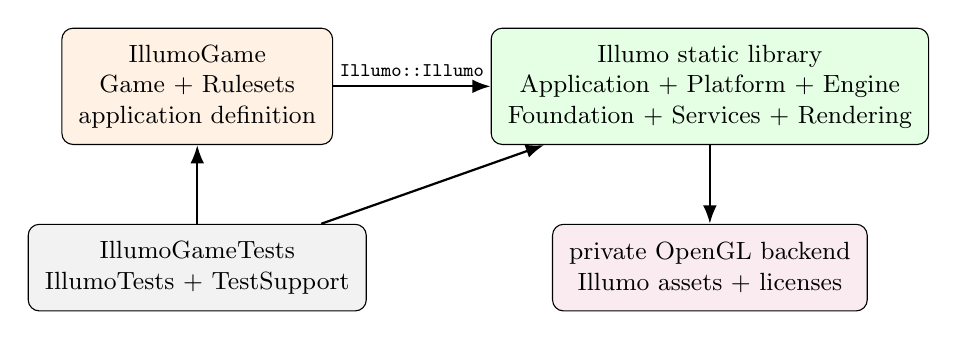
\begin{tikzpicture}[
  font=\small,
  box/.style={draw, rounded corners, align=center, inner sep=6pt, minimum height=1.1cm},
  arr/.style={-{Latex}, thick}
]
  \node[box, fill=orange!10] (game) {IllumoGame\\Game + Rulesets\\application definition};
  \node[box, fill=green!10, right=2.0cm of game] (lib) {Illumo static library\\Application + Platform + Engine\\Foundation + Services + Rendering};
  \node[box, fill=purple!8, below=1.0cm of lib] (gl) {private OpenGL backend\\Illumo assets + licenses};
  \node[box, fill=gray!10, below=1.0cm of game] (tests) {IllumoGameTests\\IllumoTests + TestSupport};

  \draw[arr] (game) -- node[above]{\scriptsize \texttt{Illumo::Illumo}} (lib);
  \draw[arr] (lib) -- (gl);
  \draw[arr] (tests) -- (game);
  \draw[arr] (tests) -- (lib);
\end{tikzpicture}
\end{center}

\subsection{Runtime one-liner}
Illumo platform entry $\rightarrow$ \symbolref{CreateIllumoApplication}
$\rightarrow$ engine-owned \symbolref{RunIllumoApplication} applies supplied
game defaults and metadata-driven CLI $\rightarrow$ construct and fallibly
initialize \symbolref{Illumo} $\rightarrow$ register the supplied required game
module and engine-owned optional Debug module $\rightarrow$ \texttt{std::chrono} loop
\{\,\symbolref{update}, \symbolref{render}\,\} until window close.

\subsection{Non-goals (current)}
\begin{itemize}
  \item No install/export package, shared DLL, or stable binary ABI.
  \item No general-purpose AAA renderer, full ECS, or speculative framework.
  \item No multiplayer or networking.
  \item No claim that Linux or macOS is supported until native validation exists.
\end{itemize}

\section{Source layout}
\label{sec:layout}

Source lives under \pathref{Illumo/Source/}. Package names describe
\textbf{responsibility}, not prestige.

\begin{table}[h]
\centering
\begin{tabularx}{\linewidth}{@{}l X@{}}
\toprule
\textbf{Package} & \textbf{Role} \\
\midrule
\pathref{App/} & Process-level app loop after OS bootstrap (\symbolref{CellMain}). \\
\pathref{Engine/} & Host: \symbolref{Illumo}, \symbolref{IModule}, context bag, Debug-only module. \\
\pathref{Game/} & Domain: canvas, cell game module, editor tools (brush/cursor). \\
\pathref{Rulesets/} & Polymorphic CA rules; \pathref{AllSets.h} umbrella for active sets. \\
\pathref{Rendering/} & Window, camera, drawables, scene, RHI-ish interfaces, OpenGL backend, Mock. \\
\pathref{Services/} & Log, env vars, input, CLI (token UI), allocators, \symbolref{SaveLoad} API. \\
\pathref{Foundation/} & Macros, build/sys info, math type aliases, small containers. \\
\pathref{Assets/} & Asset loaders (e.g.\ TTF). \\
\pathref{Platform/} & OS entry points + native dialogs / save-load. \\
\pathref{Tests/} & Granular headless suite (\texttt{IllumoTests}): game/save-load, input/services, assets, mock backend, rules, canvas, UI tokens. \\
\bottomrule
\end{tabularx}
\end{table}

\subsection{Related trees (not packages)}
\begin{itemize}
  \item \pathref{Illumo/Shader/} --- GLSL assets copied to the build tree
        (\texttt{canvas\_*.glsl}, \texttt{triangle\_*.glsl}, UI shaders).
  \item \pathref{Illumo/Assets/} --- runtime files (fonts).
  \item \pathref{Illumo/thirdparty/} --- vendored deps (GLFW, GLEW, GLM, FreeType, Tracy, \ldots).
  \item \pathref{archive/} --- historical code (old State pattern, dead render stacks). Not built.
  \item \pathref{docs/} --- all first-party documentation: current Markdown,
        package maps, dated sessions, history, one LaTeX book, and generated output.
\end{itemize}

\subsection{Naming landmine (Windows)}
\begin{decisionbox}[title={Decision: MathTypes.h (2026-07-28)}]
Do \textbf{not} put a header named \pathref{Math.h} on a case-insensitive include
path. MSVC resolves \texttt{\#include <math.h>} to it and breaks the CRT/GLM.
Project math aliases live in \pathref{Foundation/MathTypes.h}.
\end{decisionbox}

\subsection{Include style (current practice)}
\begin{statusbox}
CMake adds each package directory as an include root, so both
\texttt{"Logger.h"} and \texttt{"Services/Logger.h"} can work.
Prefer package-prefixed includes for new code so dependencies stay visible.
\end{statusbox}

\section{Runtime loop and modules}
\label{sec:runtime}

\subsection{CellMain}
\pathref{App/CellMain.cpp} owns logger init/shutdown and the frame loop:
\begin{lstlisting}
// conceptual
Logger::initLogger();
Illumo* illumo = new Illumo(argc, argv);
illumo->Init();
while (!illumo->ShouldClose()) {
  double dt = /* glfw time delta */;
  illumo->Update(dt);
  illumo->Render();
}
illumo->Shutdown();
\end{lstlisting}

\subsection{Illumo as composition root}
\symbolref{Illumo} owns the long-lived services (\symbolref{EnvVars},
\symbolref{RenderWindow}, \symbolref{Camera}, \symbolref{Renderer},
\symbolref{AssetManager}, \symbolref{CommandRegistry}, \symbolref{CommandLine},
\symbolref{InputManager}, \symbolref{Scene}) and a vector of
\symbolref{IModule} instances.

\symbolref{IllumoContext} is a \textbf{raw-pointer bag} into those services,
passed into modules at \symbolref{Start}. Ownership stays on \symbolref{Illumo}.

\begin{inferencebox}
Pattern: composition root + service locator-ish context struct (not a full
service locator library). Modules are closer to subsystems than ECS systems.
\end{inferencebox}

\subsection{IModule contract}
\begin{lstlisting}
class IModule {
public:
  virtual bool Start(IllumoContext* context) = 0;
  virtual void Update(double dt) = 0;
  virtual void DispatchDrawables(Scene* scene) = 0;
  virtual void Exit() = 0;
};
\end{lstlisting}

\begin{itemize}
  \item \textbf{Start} --- bind inputs and allocate game state; return
        \texttt{false} if required context or initialization is unavailable.
  \item \textbf{Update} --- simulation / input.
  \item \textbf{DispatchDrawables} --- contribute what should draw this frame.
  \item \textbf{Exit} --- teardown module-owned state.
\end{itemize}

\symbolref{Illumo::StartModules} erases a module whose \texttt{Start} returns
false. Only successfully started modules receive later \texttt{Update},
\texttt{DispatchDrawables}, and \texttt{Exit} calls.

Registered modules today (from \symbolref{CellMain} product composition):
\begin{itemize}
  \item \symbolref{CellGameModule} (always)
  \item \symbolref{DebugModule} (Debug configuration only; D-B1)
\end{itemize}

\begin{decisionbox}[title={D-E1 module registration}]
\pathref{Engine/Illumo.h} knows only \symbolref{IModule}.
\pathref{App/CellMain.cpp} constructs \symbolref{Illumo}, calls \texttt{Init},
registers \symbolref{CellGameModule} (and \symbolref{DebugModule} in Debug),
then \texttt{StartModules()}. Engine does not include Game headers.
\end{decisionbox}

\begin{decisionbox}[title={D-B1 Release boundary}]
\symbolref{DebugModule} is guarded twice: CMake compiles its implementation
only for Debug, and \symbolref{CellMain} includes/registers it only when
\texttt{NDEBUG} is absent. Release may share generic command/logging sources but
must not contain or construct the Debug module.
\end{decisionbox}

\subsection{Frame flow (conceptual)}
\begin{center}
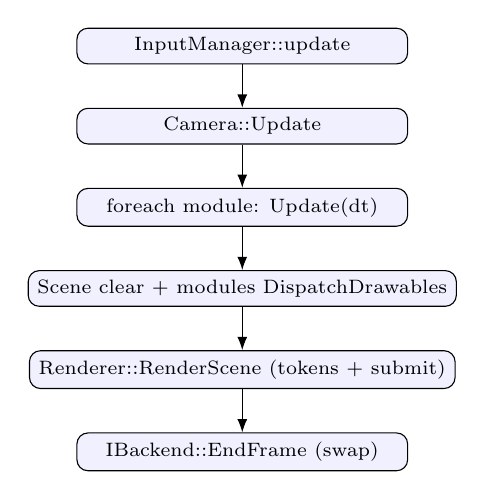
\begin{tikzpicture}[
  font=\scriptsize,
  node distance=0.55cm,
  % Do not name this style ``step'' --- it clashes with TikZ's /tikz/step key.
  flowstep/.style={draw, rounded corners, align=center, fill=blue!6, minimum width=4.2cm},
  arr/.style={-{Latex}}
]
  \node[flowstep] (1) {InputManager::update};
  \node[flowstep, below=of 1] (2) {Camera::Update};
  \node[flowstep, below=of 2] (3) {foreach module: Update(dt)};
  \node[flowstep, below=of 3] (4) {Scene clear + modules DispatchDrawables};
  \node[flowstep, below=of 4] (5) {Renderer::RenderScene (tokens + submit)};
  \node[flowstep, below=of 5] (6) {IBackend::EndFrame (swap)};
  \foreach \a/\b in {1/2,2/3,3/4,4/5,5/6} \draw[arr] (\a) -- (\b);
\end{tikzpicture}
\end{center}

\section{Rendering --- current state}
\label{sec:rendering-current}

\begin{statusbox}
\textbf{The reusable 2D renderer foundation is shipped inside Illumo.} Live
frame path is acquire/enroll + tokens + submit via
\symbolref{Renderer}/\symbolref{IBackend}.
Drawables emit tokens through \texttt{AppendCommands}; GL draw submission is
confined to \pathref{Rendering/OpenGL/} (plus window bootstrap). Headless
\pathref{Rendering/Mock/MockBackend.h} powers \texttt{IllumoTests}. CanvasView
presentation is \textbf{bounded CPU RGB fade + one RGB display texture/quad}
with dirty-rect PBO uploads (see canonical note in
\pathref{docs/architecture-consensus.md}).
No second real GPU API.
\end{statusbox}

\subsection{What actually draws frames today}
\begin{enumerate}
  \item Modules call \symbolref{DispatchDrawables} and add \symbolref{DrawableBase*}
        pointers to \symbolref{Scene} \textbf{layers}
        (\texttt{World} CanvasView, \texttt{UI} console/splash, \texttt{Debug} FPS).
  \item \symbolref{Illumo::Render} pumps completed managed asset work, then
        drives \symbolref{Renderer}:
        \texttt{BeginFrame} $\rightarrow$ \texttt{RenderScene} $\rightarrow$
        \texttt{EndFrame} (swap).
  \item \symbolref{Renderer::RenderScene}:
        one main pass --- clear + viewport tokens; walk layers
        World $\rightarrow$ UI $\rightarrow$ Debug; each drawable
        \texttt{AppendCommands}; if a drawable returns false, legacy immediate
        \texttt{Draw()} still runs (hybrid fallback; production drawables return true).
  \item \symbolref{IBackend::SubmitCommandQueue} $\rightarrow$
        \symbolref{GLDevice::ExecuteCommandQueue} resolves handles and issues GL.
\end{enumerate}

\subsection{Layers, styles, and drawables (D-R14, D-R18)}
\begin{itemize}
  \item \textbf{Layer} --- composition bucket / draw order on the default FB
        (not a multi-target GPU pass).
  \item \textbf{RenderStyle} --- Renderer-owned generational registry: shader handle +
        \texttt{PipelineState} defaults (\texttt{Canvas}, \texttt{UiText},
        \texttt{Console}, \texttt{Shape}, \texttt{Sprite}). Custom 2D styles
        use the same camera, texture, and resolution binding conventions. GPU
        programs still live in backend registries.
  \item \symbolref{DrawableBase} --- type-erased list entry; virtual
        \texttt{Draw} + virtual \texttt{AppendCommands} (default returns false).
        \textbf{No GL handle ownership} on the base (D-R6). Content handles
        only; call \texttt{bindStyle} then emit content tokens.
  \item \symbolref{Drawable<Derived>} --- CRTP: \texttt{Draw} $\rightarrow$
        \texttt{DrawImpl} for the rare immediate path. Production emitters
        (CanvasView, CommandLine, GLString/SplashText) use
        \texttt{AppendCommands} only; \texttt{DrawImpl} is empty/no-op.
  \item \symbolref{GameVisual} (D-R15) hosts composed
        shape/sprite/text values. Parent and local \texttt{Transform2D},
        normalized pivots, atlas regions/flips, and integer draw order build one
        stable cross-type stream. Only adjacent compatible items batch, so
        transparent painter order is never changed by a global texture sort.
        Dynamic buffers reserve 1,024 quads, double as needed, and stop at a
        configurable 65,536 default ceiling.
\end{itemize}

\subsection{Managed texture and shader assets (D-R17)}
\symbolref{AssetManager} caches canonical file paths plus loading options and
returns stable typed handles. Duplicate acquisition increments a reference
count; the final release destroys the backend resource. Initial pending or
failed requests retain a checkerboard texture or a fallback shader that follows
the documented custom-2D binding contract. One owned worker performs file reads
and stb decoding; \texttt{pump} applies GPU
replacement on the render thread before frame submission. Failed reloads keep
the last good object and record an error. Debug builds poll timestamps every
500\,ms and coalesce requests; explicit reload is available in all builds.
Shutdown cancels obsolete results and joins the worker before backend teardown.

\subsection{CanvasView presentation (bounded RGB fade + dirty rects)}
\label{sec:canvas-rgb-fade}
\begin{itemize}
  \item Domain: \symbolref{SparseCellGrid} stores signed-coordinate
        16$\times$16 chunks and changes its revision only for a cell-content
        change. The view visits only chunks intersecting its camera source
        bounds.
  \item View: CPU palette via \texttt{evalCell} $\rightarrow$ \texttt{targetRgb};
        \texttt{displayRgb} eases toward targets, newly revealed cells snap,
        and packed RGB is staged for upload. Unchanged grid, palette, and
        camera bounds skip resampling entirely.
  \item Zoom: normal views retain one nearest-filtered texel per 16$\times$16
        world cell. Far views use a density-colored overview bounded to about
        four screen pixels per texel; this is a visual budget, never a chunk
        or world-cell cap.
  \item GPU: one reusable nearest-filtered RGB display texture and one
        world-space quad aligned to the same 16$\times$16 cell bounds as the
        editor cursor, updated via at most one dirty-rect
        \texttt{UpdateTexture} token per submission (PBO path; optional
        \texttt{srcRowStride}). Shaders:
        \pathref{Shader/canvas\_vertex.glsl},
        \pathref{Shader/canvas\_frag.glsl} --- sample \texttt{uDisplayTexture}.
        History: D-P4 briefly used GPU R8 + $256\times 1$ palette (snap colors).
        Fade was restored; dirty-rect PBO + bind-state tracker from that work
        remain. Canonical write-up:
        \pathref{docs/architecture-consensus.md} \S5.6.
\end{itemize}

\subsection{Backend surface}
\symbolref{IBackend}: lifecycle and command-queue push/submit/clear. Resource
creation returns non-convertible slot+generation \texttt{MeshHandle},
\texttt{ShaderHandle}, and \texttt{TextureHandle} values. Validated
replace/destroy/query operations and command resolution reject stale handles
with a warning and safe no-op.

\symbolref{CommandQueue}: vector storage reserves 2,048 tokens, grows to a
configurable 65,536 default safety ceiling, and reports high-water and rejected
counts. Rejection logs once per reset interval.

\symbolref{RenderCommand}: tagged union (\texttt{CommandType} + POD payload)
including pipeline, bind, uniforms, \texttt{UpdateTexture}, \texttt{UpdateBuffer},
clear, draw, and explicit enabled/disabled scissor state (D-R1).

\symbolref{GLTexture::UpdateSubImage}: PBO ping-pong + dirty-rect packing;
fallback to client \texttt{glTexSubImage2D} if map fails.

\symbolref{GLDevice}: bind-state tracker (skip redundant program/VAO/texture/
viewport within a submit); uniform location cache; blend-func-on-enable (D-R5).
\subsection{Primitive-composed UI (D-R20)}
\begin{itemize}
  \item \symbolref{CommandLine}: one batched \texttt{UpdateBuffer} +
        \texttt{DrawIndexed} when open. Its surface, inset history, input row,
        selection, caret, scrollbar, and floating resize affordance compose
        \symbolref{GameVisual} fills, outlines, lines, and text.
  \item \symbolref{GLString}: geometry cache --- skip VBO re-upload if
        content/style unchanged (FPS $\sim$1\,Hz rebuilds). Optional panel
        chrome adds a shadow, surface, border, and accent in the same batch.
  \item \symbolref{SplashText}: fading EDIT/NORMAL label built on decorated
        GLString chrome; the two modes use distinct shared theme accents.
  \item \texttt{UiTheme}: shared value-only colors and compact panel metrics;
        it is not a retained widget tree or layout engine.
  \item \symbolref{DebugModule}: \texttt{renderer\_demo}, \texttt{assets}, and
        \texttt{asset\_reload} prove managed atlas/shader loading, atlas
        animation, transforms, tint, alpha order, async load, state inspection,
        and reload in Debug builds only.
\end{itemize}

\subsection{Tests (headless)}
Target \texttt{IllumoTests} (alias \texttt{IllumoRenderTests}) is one shared
binary for compile efficiency, but CTest invokes one exact logical case per
process (D-T1). The sparse-canvas entries cover mock/Renderer flow, assets,
rulesets, CellContext, CellGameModule commands and file-backed save/load,
CanvasView,
input/services, primitive panel composition, and UI tokens. Each case has an
isolated working directory; no
GPU context is required. The Clang/LLVM \texttt{IllumoCoverage} target enforces
85\% line coverage over headless-testable first-party production code.

\subsection{Remaining pain points (non-blocking)}
\begin{enumerate}
  \item Hybrid immediate \texttt{Draw()} remains for \emph{test stubs only};
        production drawables are pure-token (D-R10).
  \item String-named uniforms are GL-shaped debt if a second real GPU API appears
        (D-R9).
  \item \pathref{RenderWindow} still uses GLEW for context create / viewport
        (window bootstrap, not frame submission).
  \item Platform Linux/macOS render windows may still be older than the Windows path.
  \item Font atlases/UTF-8 layout, tilemaps/particles, and offscreen compositing
        are follow-on features, not hidden scaffolding in the current renderer.
\end{enumerate}

\section{Rendering --- architecture and remaining work}
\label{sec:rendering-target}

The token architecture below is the \textbf{shipped} design. Migration phases
are kept for history; treat them as complete unless a status note says otherwise.

\subsection{Goals (achieved)}
\begin{enumerate}
  \item \textbf{API isolation:} frame draw submission is via tokens; OpenGL
        execute path lives under \pathref{Rendering/OpenGL/}.
  \item \textbf{Stable front-end:} modules contribute drawables; drawables emit
        handles/uniforms/updates, not raw GL.
  \item \textbf{Record then execute:} per-frame command stream, single submit.
  \item \textbf{Resource handles:} opaque \texttt{unsigned long} table IDs;
        backend registries map to GL objects (D-R3).
  \item \textbf{Testability:} \texttt{MockBackend} + injected \symbolref{IBackend}
        (D-R7, D-R8).
\end{enumerate}

\subsection{Vocabulary}
\begin{description}[style=nextline]
  \item[Token / RenderCommand]
    A discrete instruction: bind X, set uniform Y, draw Z, update texture, \ldots
  \item[Command queue]
    Ordered buffer of tokens for the frame.
  \item[Backend]
    API-specific interpreter of tokens + owner of true GPU objects.
  \item[Enrollment]
    One-time (or rare) resource creation; returns a handle.
  \item[Front-end renderer]
    \symbolref{Renderer}: enroll helpers, push tokens, \texttt{RenderScene}.
\end{description}

\subsection{Frame pipeline (current)}

\begin{center}
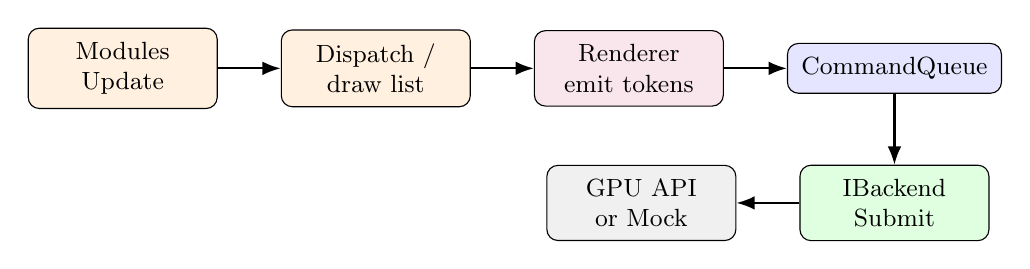
\begin{tikzpicture}[
  font=\small,
  box/.style={draw, rounded corners, align=center, inner sep=5pt, minimum width=2.4cm},
  arr/.style={-{Latex}, thick}
]
  \node[box, fill=orange!12] (mod) {Modules\\Update};
  \node[box, fill=orange!12, right=0.8cm of mod] (disp) {Dispatch /\\draw list};
  \node[box, fill=purple!10, right=0.8cm of disp] (ren) {Renderer\\emit tokens};
  \node[box, fill=blue!10, right=0.8cm of ren] (q) {CommandQueue};
  \node[box, fill=green!12, below=0.9cm of q] (be) {IBackend\\Submit};
  \node[box, fill=gray!12, left=0.8cm of be] (gpu) {GPU API\\or Mock};

  \draw[arr] (mod) -- (disp);
  \draw[arr] (disp) -- (ren);
  \draw[arr] (ren) -- (q);
  \draw[arr] (q) -- (be);
  \draw[arr] (be) -- (gpu);
\end{tikzpicture}
\end{center}

\subsection{Layering}

\begin{lstlisting}[language={}]
Game / Rulesets / UI
    |  (no gl* for draw submission)
    v
Drawable::AppendCommands(Renderer*)
    |  enroll handles + push tokens
    v
CommandQueue<RenderCommand>   // tagged union payloads
    |
    v
IBackend::SubmitCommandQueue
    |
    +-- GLBackend + GLDevice   (production: CreateOpenGLBackend at Illumo::Init)
    +-- MockBackend            (tests inject; takeOwnership=false)

Renderer.h depends only on IBackend*; OpenGL types stay under Rendering/OpenGL/.
\end{lstlisting}

\subsection{Drawable meaning}
``Drawable'' means \emph{something that can append tokens} (and optionally fall
back to immediate \texttt{Draw}). GL objects live in backend registries, not on
\symbolref{DrawableBase}.

CanvasView end state (shipped):
\begin{itemize}
  \item Domain: \texttt{SparseCellGrid}, signed coordinates, 16$\times$16
        chunks, and serial 18$\times$18 halo stepping.
  \item View: bounded camera sampling + RGB fade buffers + one RGB display
        texture and one screen-space quad; linear display sampling avoids
        nearest-neighbor blockiness when zoomed out, while dirty-rect
        \texttt{UpdateTexture} remains the only per-frame texture upload
        (PBO).
  \item See \pathref{docs/architecture-consensus.md} for the single canonical
        presentation model (R8-only notes are historical).
\end{itemize}

\subsection{Migration phases (historical checklist)}
\label{sec:migration-phases}

\begin{enumerate}[leftmargin=*]
  \item \textbf{Phase 0 --- Document \& freeze vocabulary} \quad \textbf{done}
  \item \textbf{Phase 1 --- Token proof path} \quad \textbf{done}
        (\texttt{RenderProofQuad}, tagged union, mesh upload, handle resolve)
  \item \textbf{Phase 2 --- Scene through Renderer} \quad \textbf{done}
  \item \textbf{Phase 3 --- Canvas tokens} \quad \textbf{done}
        (later: dirty-rect uploads; D-P4 R8 experiment then fade restore)
  \item \textbf{Phase 4 --- UI drawables} \quad \textbf{done}
        (GLString, CommandLine, SplashText)
  \item \textbf{Phase 5 --- Dead path cleanup} \quad \textbf{done}
        (archive under \pathref{archive/dead-render/}; pure DrawableBase)
  \item \textbf{Phase 6 --- Mock backend} \quad \textbf{done}
        (no second real API yet)
\end{enumerate}

\subsection{Acceptance criteria (migration ``done'')}
\begin{itemize}
  \item[\checkmark] Frame path is enroll + token queue + submit.
  \item[\checkmark] Cell sim runs: edit, step/rules, camera, console, FPS, splash.
  \item[\checkmark] \symbolref{Renderer::RenderScene} is non-empty and used.
  \item[\checkmark] Mock/headless tests cover tokens and domain.
  \item Partial: \texttt{gl*} still appears in window bootstrap and
        \pathref{Rendering/OpenGL/}; some non-Windows platforms lag.
\end{itemize}

\subsection{Optional future work}
\begin{itemize}
  \item Generational handles / explicit destroy beyond shutdown-only (D-R4).
  \item Second real graphics API (only if needed).
  \item GPU color fade without bringing back full-grid float RGB.
  \item Further slim \symbolref{Renderer} so production does not include GL headers
        in the public header (pimpl / factory).
  \item Linux/macOS parity with the Windows token path.
\end{itemize}

\section{Game domain and rulesets}
\label{sec:game}

\subsection{CellGameModule}
Primary gameplay module. Owns a \symbolref{CellContext} and an enum
\symbolref{CellState}:
\begin{center}
\texttt{NORMAL} $\mid$ \texttt{EDIT} $\mid$ \texttt{EXIT}
\end{center}

\begin{statusbox}
Mode handling is an \textbf{enum + switch} inside the module, not the older
class-per-state hierarchy (archived under \pathref{archive/old-states/}).
\texttt{E} toggles EDIT/NORMAL and wakes \symbolref{SplashText}.
Save/load, pause/run/step, canvas, ruleset, and camera behavior is exposed as
registered console commands rather than artificial frame states.
Simulation rate: env \texttt{tps} $\times$ \texttt{speedFactor}, with
accumulator + step cap. Painting and simulation operate on signed world
coordinates; there is no finite or toroidal production canvas.
\end{statusbox}

\subsection{Domain console commands and persistence}
\symbolref{CellGameModule} registers domain commands through
\symbolref{CommandRegistry}; Services remains free of Game types. Save always
writes version 2 sparse files with magic/version, ruleset, camera metadata, and
sorted 16$\times$16 chunk records. Load validates temporary state before
mutation, accepts both version 2 and the prior dense format, imports legacy
cells around the origin, restores ruleset/camera metadata, and snaps the
bounded view. Native picker variants route through the platform
\symbolref{SaveLoad} API. See D-CLI1 and
\cref{sec:session-2026-08-04}.

\subsection{CellContext}
Constructs \symbolref{SparseCellGrid} and bounded \symbolref{CanvasView} from
env vars (\texttt{CanvasX}, \texttt{CanvasY}) and selects a \symbolref{RuleSet}
from a mode string
(\texttt{GAME\_OF\_LIFE}, \texttt{BRIANS\_BRAIN}, \texttt{SEEDS}, \ldots).
Mode changes from console/env call \texttt{setRuleSet} and
\texttt{CanvasView::rebuildPalette}.

\subsection{SparseCellGrid (domain) and CanvasView (view --- D-C3)}
\begin{itemize}
  \item Domain: signed 64-bit cell addresses map through floor division into
        non-background 16$\times$16 byte chunks. Negative coordinates and all
        multi-state values are preserved; no fixed chunk pool cap exists.
  \item Simulation: active chunks plus their neighbors are read through a
        temporary 18$\times$18 halo and stepped serially with stateless
        \texttt{RuleSet::nextState}; empty space is implicit and non-toroidal.
  \item View: \symbolref{CanvasView} samples the camera-visible region into a
        bounded RGB staging buffer, fades palette colors, and snaps newly
        revealed cells.
  \item GPU: one reusable RGB display texture and one screen-space
        \symbolref{GameVisual} quad; at most one dirty texture update per view
        submission.
  \item Dense \symbolref{CellGrid}/\symbolref{Canvas} remains only for
        compatibility tests and legacy import, not as a second runtime path.
\end{itemize}

\subsection{Scale walls (simulation / memory)}
\begin{statusbox}
Simulation cost follows allocated chunks and their eight-neighbor halo set,
not a fixed world rectangle. Presentation cost follows the bounded
\texttt{CanvasX}$\times$\texttt{CanvasY} view. GPU resources do not scale with
chunk count.
\end{statusbox}

\subsection{Rulesets}
Active rules (in \pathref{AllSets.h} / factory): Game of Life, Seeds, Brian's
Brain, Highlife, Day \& Night, Life Without Death, Wireworld. Stub headers
remain for Rule 90 / 184 (identity \texttt{nextState}).

\begin{lstlisting}
class RuleSet {
  // Pure transition: cell + Moore count of alive (value==0) neighbors.
  virtual unsigned char nextState(unsigned char cell,
                                  unsigned char aliveNeighbors) const;
  virtual void evalCell(const unsigned char& target,
                        unsigned char dest[3]) const; // palette colors
};
\end{lstlisting}

\textbf{Generation:}
\begin{enumerate}
  \item Collect every allocated chunk and its eight neighboring chunk
        addresses.
  \item Fill a temporary 18$\times$18 read-only halo for each target chunk.
  \item Evaluate the 16$\times$16 core and install only non-background chunks.
\end{enumerate}

\begin{decisionbox}[title={Keep rules pure}]
Rulesets stay free of rendering and input. They read/write cell buffers only
and expose \texttt{evalCell} for palette colors. That keeps them testable
(headless \texttt{TestRuleSets}).
\end{decisionbox}

\subsection{Cell encoding}
\begin{center}
\begin{tabular}{@{}ll@{}}
\toprule
\textbf{Value} & \textbf{Meaning} \\
\midrule
$0$ & Alive / Wireworld head (neighbor count treats as ``live'') \\
$1$ & Dead / Wireworld empty \\
$2$ & Multi-state (Brian's Brain dying; Wireworld tail) \\
$3$ & Wireworld conductor \\
\bottomrule
\end{tabular}
\end{center}
Historical neighbor tests used \texttt{!getCanvasPixel} (alive when zero).
Wireworld reuses head $=0$ so head-neighbor counting stays simple.

\section{Services, foundation, platform}
\label{sec:services}

\subsection{Services}
Cross-cutting facilities used by Engine/Game/Rendering:
\begin{itemize}
  \item \textbf{Logging} --- \symbolref{Logger} (file + terminal; level from env).
  \item \textbf{Config} --- \symbolref{EnvVars} / \symbolref{IEnvVars}
        (defaults filled in \symbolref{Illumo::Init}: canvas size, fps/tps,
        synchronized presentation via \texttt{vsync}, mode string, \ldots).
        The production file is \texttt{envvars.json}
        beside the executable, seeded from the tracked default only when absent;
        it never depends on the launch working directory.
  \item \textbf{Input} --- \symbolref{InputManager}, \symbolref{InputContext},
        \symbolref{KeyCode}; action binding used by the game module.
        No Game types (D-E2).
  \item \textbf{CLI} --- \symbolref{CommandLine} owns the token UI and batched
        geometry. \symbolref{CommandRegistry} owns command metadata and
        callbacks; \symbolref{SysCmdLine} handles startup options. Help,
        version, and window/canvas dimensions are applied before window creation.
        General tooling stays in Services; \symbolref{CellGameModule} registers
        simulation/canvas/camera/save-load commands with usage, descriptions,
        and completion candidates. Editing includes selection, word movement and
        deletion, history, quoted arguments, measured caret placement, command
        chaining with \texttt{;}, alias macro management (\texttt{alias}/\texttt{unalias}),
        inline ghost-text auto-suggestions, dynamic parameter hints, and a
        horizontally scrolling input viewport. The current history draw path
        truncates each entry to panel width and scrolls by raw history entries;
        D-UI2's word-wrap and visual-line metrics are not currently
        implemented. The easy-font batch is sized for 8,000 UI quads. The
        console is Debug-only product composition
        (D-B1, D-CLI1, D-UI1--D-UI3).
  \item \textbf{Allocators} --- pool/arena/debug allocators (experimental /
        learning surface; not all wired into the hot path).
  \item \textbf{SaveLoad API} --- pure declarations; OS dialogs implemented
        per platform.
\end{itemize}

\subsection{Foundation}
Headers that should stay cheap to include:
macros (\pathref{MacroDefs.h}), build info, \pathref{MathTypes.h},
\pathref{ArrayQueue.h}.

\begin{statusbox}
\pathref{MacroDefs.h} still pulls Windows headers on \texttt{\_WIN32} (for
\texttt{Sleep} / \texttt{\_\_SLEEP}). That is include-heavy for a widely used
header. \textbf{Deferred (D-F1):} leave as-is until compile time, name
collisions, or header hygiene actually hurt; then split platform sleep into a
narrower header.
\end{statusbox}

\subsection{Platform}
Thin platform sources:
\begin{itemize}
  \item Windows: \pathref{WinMain.cpp}, \pathref{WinSaveLoad.cpp} ---
        supported and currently verified.
  \item Linux: \pathref{\_main.cpp}, \pathref{LinuxSaveLoad.cpp}
        --- unsupported stale scaffold; the entry references removed shared
        bootstrap APIs.
  \item macOS: \pathref{Main.cpp}, \pathref{MacSaveLoad.mm}
        --- unsupported stale scaffold; the entry references removed APIs and
        CMake does not enable Objective-C++ for the selected \texttt{.mm} file.
\end{itemize}

Contract: bootstrap $\rightarrow$ call \symbolref{CellMain}. Each port also
implements the native load-location and save-location functions in
\symbolref{SaveLoad}.
Source presence and CMake selection do not establish support; Linux/macOS
require native configure, build, tests, rendering/input, dialogs, and shutdown
validation.

\subsection{Third-party}
Vendored under \pathref{Illumo/thirdparty/}. Policy from \pathref{docs/contributing.md}:
new third-party deps require review/PR. Existing: GLFW, GLEW, GLM, FreeType,
JSON, STB, Tracy, image libs, \ldots

\section{Design decision log}
\label{sec:decisions}

Append-only log. Newest entries at the bottom. If a decision is reversed, add a
new entry that supersedes the old id; do not silently delete history.

%----------------------------------------------------------------------------
\subsection*{D-001 --- Package rename (structure)}
\begin{decisionbox}[title={D-001 \quad 2026-07-28}]
\textbf{Decision:} Rename/split ambiguous folders to match responsibility:
\texttt{Core$\rightarrow$Game}, \texttt{System$\rightarrow$\{App,Engine,Services\}},
\texttt{Init+Util$\rightarrow$Foundation}, \texttt{AssetLoaders$\rightarrow$Assets}.\\
\textbf{Why:} Names were lying; slowed reasoning and migrations.\\
\textbf{Consequences:} Include/CMake paths updated; archive for old States.
\end{decisionbox}

%----------------------------------------------------------------------------
\subsection*{D-002 --- MathTypes header name}
\begin{decisionbox}[title={D-002 \quad 2026-07-28}]
\textbf{Decision:} Project math aliases live in \pathref{MathTypes.h}, not
\pathref{Math.h}.\\
\textbf{Why:} Windows case-insensitive include collision with CRT
\texttt{math.h}.\\
\textbf{Consequences:} All includes updated; the Foundation package map under
\pathref{docs/packages/} notes the trap.
\end{decisionbox}

%----------------------------------------------------------------------------
\subsection*{D-003 --- Render abstraction direction}
\begin{decisionbox}[title={D-003 \quad 2026-07-28 (implemented; see D-R*) }]
\textbf{Decision:} Command/token submission via \symbolref{IBackend}
+ \symbolref{RenderCommand} queue; game code must not permanently depend on
raw GL for draw submission.\\
\textbf{Why:} Multi-API optionality; clearer frame boundary; testability.\\
\textbf{Consequences:} Phases 1--6 complete for planned scope
(\cref{sec:migration-phases}); hybrid immediate \texttt{Draw} remains only as
fallback.
\end{decisionbox}

%----------------------------------------------------------------------------
\subsection*{D-004 --- Module frame hooks}
\begin{decisionbox}[title={D-004 \quad inferred from IModule}]
\textbf{Decision:} Modules expose \symbolref{Start}/\symbolref{Update}/
\symbolref{DispatchDrawables}/\symbolref{Exit}.\\
\textbf{Why:} Separate simulation tick from draw contribution.\\
\textbf{Consequences:} Draw list is rebuilt or contributed each frame through
dispatch. Module ownership/composition was later closed by D-E1.
\end{decisionbox}

%----------------------------------------------------------------------------
\subsection*{D-005 --- Rules as polymorphic sets}
\begin{decisionbox}[title={D-005 \quad inferred}]
\textbf{Decision:} Each CA variant is a \symbolref{RuleSet} subclass.\\
\textbf{Why:} Open for extension; shared generation sweep.\\
\textbf{Consequences:} Factory logic currently in \symbolref{CellContext}
string matching (could become a registry later).
\end{decisionbox}

%----------------------------------------------------------------------------
\subsection*{D-006 --- Mode handling (enum vs State classes)}
\begin{decisionbox}[title={D-006 \quad current code; author may supersede}]
\textbf{Decision (current):} \symbolref{CellState} enum inside
\symbolref{CellGameModule}.\\
\textbf{Supersedes:} class hierarchy under \pathref{archive/old-states/}.\\
\textbf{Why (inferred):} fewer types for a small mode set.\\
\textbf{Open at decision time:} SAVE/LOAD completeness; whether splash/global
state is acceptable.\\
\textbf{Resolution (2026-08-04):} frame modes are now
\texttt{NORMAL | EDIT | EXIT}; save/load are registered commands with validated
file handling (D-CLI1).
\end{decisionbox}

%----------------------------------------------------------------------------
\subsection*{D-007 --- Enrollment vs per-frame commands}
\begin{decisionbox}[title={D-007 \quad visible in Renderer comments}]
\textbf{Decision:} Resource creation goes through enroll/Create* APIs; do not
stuff mesh/shader creation into the per-frame token stream.\\
\textbf{Why:} Keep the frame queue about \emph{binding and drawing}.\\
\textbf{Consequences:} Need an explicit destroy/reload story for hot-reload
later.
\end{decisionbox}

%----------------------------------------------------------------------------
\subsection*{D-008 --- contributing constraints}
\begin{decisionbox}[title={D-008 \quad from docs/contributing.md}]
\textbf{Decision:} Avoid \texttt{auto}; avoid namespaces (prefer static
classes/structs); no recursion; third-party via PR.\\
\textbf{Why:} Author house style / learning constraints.\\
\textbf{Consequences:} Documentation and new code should respect these unless
explicitly waived in a later decision.
\end{decisionbox}

%----------------------------------------------------------------------------
\subsection*{D-R1 --- RenderCommand payload shape}
\begin{decisionbox}[title={D-R1 \quad 2026-07-28}]
\textbf{Decision:} \symbolref{RenderCommand} uses a \textbf{simple tagged union}
(\texttt{CommandType} + POD payload union), not a kitchen-sink flat struct and
not a byte-stream compiler. Prefer C-style union over \texttt{std::variant}.\\
\textbf{Why:} Type-safe uniforms/clear/update data while remaining
copyable for \symbolref{ArrayQueue}; matches house style.\\
\textbf{Consequences:} \pathref{Rendering/RenderCommand.h} redesigned; execute
path switches on type and reads the matching payload.
\end{decisionbox}

%----------------------------------------------------------------------------
\subsection*{D-R2 --- Who emits tokens}
\begin{decisionbox}[title={D-R2 \quad 2026-07-28}]
\textbf{Decision:} Each drawable emits its own tokens via
\texttt{AppendCommands(Renderer*)} (or equivalent). \symbolref{Renderer}
owns frame setup (clear/viewport) and submit.\\
\textbf{Why:} Smallest strangler step from today's
\symbolref{DispatchDrawables} list.\\
\textbf{Consequences:} Hybrid phase may still call immediate \texttt{Draw}
for unmigrated drawables after token submit.
\end{decisionbox}

%----------------------------------------------------------------------------
\subsection*{D-R3 --- Handle typing for v1}
\begin{decisionbox}[title={D-R3 \quad 2026-07-28}]
\textbf{Decision:} Keep \texttt{unsigned long} opaque handles with backend
registries (\texttt{tableID} $\rightarrow$ GL object). Strong typedefs deferred.\\
\textbf{Why:} Minimal churn; critical fix is resolve-on-submit, not type names.\\
\textbf{Consequences:} Execute must never treat handles as raw GLuints without
registry lookup.
\end{decisionbox}

%----------------------------------------------------------------------------
\subsection*{D-R4 --- Migration scope}
\begin{decisionbox}[title={D-R4 \quad 2026-07-28}]
\textbf{Decision:} Full migration Phases 1--5 (token proof $\rightarrow$ Scene
routing $\rightarrow$ Canvas $\rightarrow$ UI drawables $\rightarrow$ cleanup).
Phase 6 (mock backend) included; second real GPU API still optional.\\
\textbf{Why:} Playable strangler path to API isolation without big-bang rewrite.\\
\textbf{Also freeze for v1:} destroy resources at shutdown only; Windows GL is
primary platform.\\
\textbf{Superseded in part by D-P1/D-P4:} full-frame Canvas rewrite was v1 only.
Dirty-rect/PBO uploads remain, while the R8 presentation was later superseded
by the restored RGB fade path documented in D-P4.
\end{decisionbox}

%----------------------------------------------------------------------------
\subsection*{D-R5 --- Blend state on first enable}
\begin{decisionbox}[title={D-R5 \quad 2026-07-28}]
\textbf{Decision:} When enabling blending in \symbolref{GLDevice::ApplyPipelineState},
always call \texttt{glBlendFunc} (do not rely on CPU-side factor cache matching
defaults).\\
\textbf{Why:} OpenGL default is \texttt{ONE}/\texttt{ZERO}; cache defaults were
SrcAlpha/OneMinusSrcAlpha so factors looked ``unchanged'' and console panel
lost transparency after the token migration.\\
\textbf{Consequences:} Semi-transparent UI (console panel alpha) works again.
\end{decisionbox}

%----------------------------------------------------------------------------
\subsection*{D-R6 --- Dead stack cleanup (Phase 5)}
\begin{decisionbox}[title={D-R6 \quad 2026-07-28}]
\textbf{Decision:} Archive window \symbolref{RenderQueue}, legacy
\texttt{Drawable.cpp} GL helpers, empty \texttt{Transform}/\texttt{RenderContext},
and unused \texttt{CellCommandLine} under \pathref{archive/dead-render/}.
\symbolref{DrawableBase} is a pure list/token interface (no GL handles).\\
\textbf{Why:} Token path won; dual submission models confuse maintenance.\\
\textbf{Consequences:} \texttt{IRenderWindow::getRenderQueue} removed; frame
draw list is only \symbolref{Scene} + \symbolref{Renderer}.
\end{decisionbox}

%----------------------------------------------------------------------------
\subsection*{D-R7 --- Mock backend for tests (Phase 6)}
\begin{decisionbox}[title={D-R7 \quad 2026-07-28}]
\textbf{Decision:} Add headless \texttt{MockBackend} implementing
\symbolref{IBackend}: record \texttt{Create*} and snapshot the command queue
on \texttt{SubmitCommandQueue}. Originally shipped as CMake target
\texttt{IllumoRenderTests} / CTest \texttt{MockBackend}; the current canonical
target and CTest name are \texttt{IllumoTests}, with the old names retained only
as compatibility aliases. Do \textbf{not} add Vulkan/Metal yet.\\
\textbf{Why:} First meaningful automated render test without a GPU context;
proves token vocabulary and handle plumbing independently of GL.\\
\textbf{Consequences:} CI can run \texttt{ctest -R IllumoTests}; second real API
remains future work after more production needs appear.
\end{decisionbox}

%----------------------------------------------------------------------------
\subsection*{D-R8 --- Inject IBackend into Renderer}
\begin{decisionbox}[title={D-R8 \quad 2026-07-28, refined 2026-08-07}]
\textbf{Decision:} \symbolref{Renderer} is backend-neutral: its only constructor
takes an injected \symbolref{IBackend*} and a \texttt{takeOwnership} flag.
Production composition (\symbolref{Illumo}\texttt{::Init}) constructs the real
backend via \texttt{CreateOpenGLBackend} under \pathref{Rendering/OpenGL/} and
injects it with \texttt{takeOwnership=true}. Tests inject \texttt{MockBackend}
with \texttt{takeOwnership=false}. \texttt{Renderer.h} must not include or
construct concrete OpenGL types.\\
\textbf{Why:} End-to-end drawable $\rightarrow$ enroll/token $\rightarrow$ submit
without a GPU; second platforms can supply a different \symbolref{IBackend}
without touching the generic frame-submit surface.\\
\textbf{Consequences:} \texttt{TestRendererE2E} covers inject, owned-backend
composition style, header neutrality, \texttt{RenderScene}, Canvas tokens,
hybrid immediate drawables, and \texttt{RenderProofQuad}. OpenGL sources stay
under \pathref{Rendering/OpenGL/}; Mock under \pathref{Rendering/Mock/}.
\end{decisionbox}

%----------------------------------------------------------------------------
\subsection*{D-P1 --- Dirty visual path}
\begin{decisionbox}[title={D-P1 \quad 2026-07-28}]
\textbf{Decision:} Canvas/CellGameModule use dirty flags so idle frames skip
full-grid visual work and GPU upload.\\
\textbf{Why:} Dominant cost was recoloring + full texture upload every render
frame even when the CA did not step.\\
\textbf{Consequences:} \texttt{cellsDirty}, upload pending, early-out
\texttt{tickVisual}; still life after sim step does not re-dirty.
\end{decisionbox}

%----------------------------------------------------------------------------
\subsection*{D-P2 --- UI batching and geometry cache}
\begin{decisionbox}[title={D-P2 \quad 2026-07-28}]
\textbf{Decision:} CommandLine emits one packed \texttt{UpdateBuffer}/draw when
open; GLString caches GPU geometry until content/style changes.\\
\textbf{Why:} Per-line uploads and FPS string rebuilds were measurable when the
console/FPS overlay was active.\\
\textbf{Consequences:} Token stream stays small; FPS may rebuild $\sim$1\,Hz.
\end{decisionbox}

%----------------------------------------------------------------------------
\subsection*{D-P3 --- Double-buffer CA generation}
\begin{decisionbox}[title={D-P3 \quad 2026-07-28}]
\textbf{Decision:} \texttt{RuleSet::calcGeneration} writes pure
\texttt{nextState(cell, aliveNeighbors)} into a scratch buffer, then
\texttt{memcpy}s back; neighbor counts use raw grid pointers + toroidal wrap.\\
\textbf{Why:} Correct simultaneous update; faster than per-cell
\texttt{getCanvasPixel}/in-place virtual writes; sparse dirty AABB for visuals.\\
\textbf{Consequences:} All active rulesets override \texttt{nextState}; stubs
use identity.\\
\textbf{Refined by D-P5 (2026-08-06):} scratch lives on \symbolref{CellGrid}
as a back buffer; promotion is pointer swap, not full-grid \texttt{memcpy}.
\end{decisionbox}

%----------------------------------------------------------------------------
\subsection*{D-P5 --- Single-pass dirty AABB + buffer swap}
\begin{decisionbox}[title={D-P5 \quad 2026-08-06}]
\textbf{Decision:} Track changed-cell AABB during the eval pass; store next
generation in \texttt{CellGrid} back buffer; on any change call
\texttt{swapLifeBuffers()} and mark the sparse dirty region. Interior Moore
counts skip toroidal wrap branches.\\
\textbf{Why:} Second full-grid compare pass and full \texttt{memcpy} write-back
dominated serial generation cost on large dense grids.\\
\textbf{Consequences:} \texttt{lifeCanvas} always means current front; rules
must not retain raw pointers across a swap; still life leaves domain clean.
\end{decisionbox}

%----------------------------------------------------------------------------
\subsection*{D-P6 --- Fade loop + packed dirty PBO staging}
\begin{decisionbox}[title={D-P6 \quad 2026-08-06}]
\textbf{Decision:} Keep CPU RGB fade presentation. Hoist coordinates in
\texttt{tickVisual}/\texttt{snapVisualToTargets}; rectangular target rebuild
uses one \texttt{includeRect}. \texttt{GLTexture::UpdateSubImage} packs partial
dirty rects tightly and maps only the staging range (no full-buffer orphan
every frame).\\
\textbf{Why:} Per-cell div/mod and full-texture PBO orphan were measurable on
large dirty rects while fade quality must stay.\\
\textbf{Consequences:} Fade math unchanged; MockBackend token path unaffected.
\end{decisionbox}

%----------------------------------------------------------------------------
\subsection*{D-P7 --- Optional row-parallel generation}
\begin{decisionbox}[title={D-P7 \quad 2026-08-06}]
\textbf{Decision:} \texttt{RuleSet::calcGeneration} may partition rows across
workers when cell count $\ge 512\times 512$ (auto) or when
\texttt{setWorkerOverride(N)} forces $N$ workers. Results are bit-identical to
serial. Presentation/fade stays main-thread.\\
\textbf{Why:} Large dense grids are eval-bound after D-P5; spawn cost makes
parallel unhelpful on default $80\times 60$.\\
\textbf{Consequences:} Tests cover serial/parallel identity
(\texttt{Illumo.Sim.SerialParallelIdentical}); micro-benches under
\texttt{Illumo.Sim.MicroBench}. Persistent thread pool deferred.
\end{decisionbox}

%----------------------------------------------------------------------------
\subsection*{D-P4 --- dirty-rect PBO uploads (R8 path partially superseded)}
\begin{decisionbox}[title={D-P4 \quad 2026-07-28}]
\textbf{Decision (original):} Present cells as \texttt{GL\_R8} texture of state
bytes plus a $256\times 1$ RGB palette (\texttt{evalCell}). Upload dirty rects
via PBO ping-pong in \texttt{GLTexture::UpdateSubImage}. Drop dual float RGB
staging.\\
\textbf{Why:} Large grids: bandwidth and CPU of RGB float fade dominated.\\
\textbf{Consequences (kept):} dirty-rect \texttt{UpdateTexture}, PBO path,
bind-state tracker in \symbolref{GLDevice}.\\
\textbf{Superseded presentation (2026-07-30):} live path restored to CPU RGB
fade (\texttt{targetRgb}/\texttt{displayRgb}) + RGB display texture so cell
colors ease rather than snap. R8+palette is historical experiment, not current
code truth. Canonical: \pathref{docs/architecture-consensus.md}.
\end{decisionbox}

%----------------------------------------------------------------------------
\subsection*{D-E1 --- Module registration lives in App}
\begin{decisionbox}[title={D-E1 \quad 2026-07-28}]
\textbf{Decision:} \symbolref{Illumo} does not include or construct
\symbolref{CellGameModule}. \pathref{App/CellMain.cpp} calls \texttt{Init},
\texttt{addModule}, then \texttt{StartModules}. Debug module is registered
from App under \texttt{\#ifndef NDEBUG}.\\
\textbf{Why:} Engine must not depend on Game headers; product composition
belongs at the application boundary.\\
\textbf{Consequences:} New products/tests can register different module sets;
Engine only knows \symbolref{IModule}.
\end{decisionbox}

%----------------------------------------------------------------------------
\subsection*{D-E2 --- InputManager has no Game types}
\begin{decisionbox}[title={D-E2 \quad 2026-07-28}]
\textbf{Decision:} Remove \texttt{CellContext*} and Game includes from
\symbolref{InputManager}. Also drop unused \texttt{SplashText} extern from the
input header.\\
\textbf{Why:} Services must not depend on Game; input is a pure device/action
service. Splash and rules stay in Game/Rendering.\\
\textbf{Consequences:} InputManager header only needs KeyCode/InputContext/GLFW.
\end{decisionbox}

%----------------------------------------------------------------------------
\subsection*{D-E3 --- EntityTable is not the cell path}
\begin{decisionbox}[title={D-E3 \quad 2026-07-28}]
\textbf{Decision:} Archive \pathref{EntityTable.h} and \pathref{ModuleObject.h}
under \pathref{archive/dead-engine/}. Remove \texttt{entityTable} from
\symbolref{Scene}/\symbolref{IllumoContext}.\\
\textbf{Why:} Nothing allocated or used an EntityTable; the live path is
drawables + tokens, not ECS.\\
\textbf{Consequences:} Reintroduce a general object table only when a real
feature needs it; document that cells are not entities.
\end{decisionbox}

%----------------------------------------------------------------------------
\subsection*{D-E4 --- Scene is a drawable list, not a graph}
\begin{decisionbox}[title={D-E4 \quad 2026-07-28}]
\textbf{Decision:} \symbolref{Scene} holds only \texttt{drawables},
\texttt{window}, and \texttt{activeCamera}. Remove \texttt{root},
\texttt{nodeLookup}, no-op \texttt{Update}, and unused
\texttt{RenderableObject}. Archive \pathref{SceneObject.h}; \symbolref{Camera}
and \symbolref{CommandLine} no longer inherit a node graph.\\
\textbf{Why:} Architecture review (dead graph scaffolding); production never
used parent/child transforms for cells or UI.\\
\textbf{Consequences:} Frame contribution model is explicit and small.
\end{decisionbox}

%----------------------------------------------------------------------------
\subsection*{D-E5 --- Freeze IllumoContext; validate at Start}
\begin{decisionbox}[title={D-E5 \quad 2026-07-28}]
\textbf{Decision:} Keep \symbolref{IllumoContext} as a service bag for the
\textbf{two shipped modules} only. Document required fields per module.
\texttt{Start()} logs an error and bails if the bag is incomplete.
Do not grow the bag for convenience; a third module should take explicit
constructor dependencies if its subset differs.\\
\textbf{Why:} Architecture review --- bag cost is zero at $N=2$ but becomes a
de-facto global API as $N$ grows.\\
\textbf{Consequences:} \texttt{IllumoContextHasGameCore} /
\texttt{IllumoContextHasDebugCore} helpers; freeze note on the struct.
\end{decisionbox}

%----------------------------------------------------------------------------
\subsection*{D-C1 --- Canvas dual role is intentional (for now)}
\begin{decisionbox}[title={D-C1 \quad 2026-07-28}]
\textbf{Decision:} Keep \symbolref{Canvas} as domain grid + fade view + GPU
enroll in one type. Document the scale wall: full-grid
\texttt{calcGeneration}, dual float RGB buffers ($\sim$24\,B/cell), no
chunked simulation domain.\\
\textbf{Why:} Locality for dirty-rect + palette + fade; headless tests already
use injected MockBackend rather than pure LifeGrid.\\
\textbf{Consequences:} Split \texttt{LifeGrid}/\texttt{CanvasView} only if pure
sim tests or large canvases become product requirements.
\end{decisionbox}

%----------------------------------------------------------------------------
\subsection*{D-R9 --- String-named uniforms are backend debt}
\begin{decisionbox}[title={D-R9 \quad 2026-07-28}]
\textbf{Decision:} Keep \texttt{char name[32]} uniforms for OpenGL + Mock.
Treat as debt if a second \emph{real} GPU backend is adopted; prefer binding
points / pre-resolved locations then.\\
\textbf{Why:} Architecture review --- uniform path is the least portable part
of \symbolref{RenderCommand}; handles and UpdateTexture are closer to neutral.\\
\textbf{Consequences:} Comment on uniform payloads; no API change now.
\end{decisionbox}

%----------------------------------------------------------------------------
\subsection*{D-R10 --- Production drawables are pure-token}
\begin{decisionbox}[title={D-R10 \quad 2026-07-28}]
\textbf{Decision:} \symbolref{Canvas}, \symbolref{CommandLine},
\symbolref{GLString}, \symbolref{SplashText} use
\texttt{AppendCommands} only (return true when contributing). Immediate
\texttt{Draw()} hybrid remains for tests/stubs. CRTP \texttt{DrawImpl} is
legacy for that fallback.\\
\textbf{Why:} Migration complete for shipped UI/canvas; dual path is debt only
where unmigrated types exist.\\
\textbf{Consequences:} Documented in \pathref{Drawable.h} and
\texttt{Renderer::RenderScene}.
\end{decisionbox}

%----------------------------------------------------------------------------
\subsection*{D-R14 --- Scene layers and built-in render styles}
\begin{decisionbox}[title={D-R14 \quad 2026-08-07}]
\textbf{Decision:} Introduce \textbf{Phase A} composition without multi-pass
GPU targets:
\begin{itemize}
  \item \symbolref{Scene} buckets drawables into ordered layers
        (\texttt{World}, \texttt{UI}, \texttt{Debug}) within one main pass
        (default framebuffer, single clear).
  \item \symbolref{Renderer} owns built-in \symbolref{RenderStyle} entries
        (\texttt{Canvas}, \texttt{UiText}, \texttt{Console}): each holds a
        shader table handle plus \texttt{PipelineState} defaults.
  \item Production drawables keep content handles (mesh/texture/domain data)
        and call \texttt{bindStyle} before content tokens.
\end{itemize}
Layers are not the same as \symbolref{RenderPass} (targets/load-store). A
layer may later feed multiple passes if targets diverge; that is deferred.\\
\textbf{Why:} World/UI/debug stacking and shared draw policy should not live
as duplicated per-drawable shader enrollment and ad-hoc pipeline structs.\\
\textbf{Consequences:} \pathref{RenderLayerId.h}, \pathref{RenderStyle.h},
\pathref{RendererStyles.cpp}; modules pass a layer to
\texttt{Scene::AddDrawable}; docs distinguish layer vs pass.
\end{decisionbox}

%----------------------------------------------------------------------------
\subsection*{D-R15 --- Render primitives and GameVisual host}
\begin{decisionbox}[title={D-R15 \quad 2026-08-07}]
\textbf{Decision:} Introduce value-type \textbf{render primitives}
(\symbolref{ShapePrimitive}, \symbolref{SpritePrimitive}) composed on a
\symbolref{GameVisual} \texttt{Drawable} host.
\begin{itemize}
  \item Primitives are not Scene entries; the host is.
  \item Game/editor objects \textbf{embed} \symbolref{GameVisual} (or multiple)
        and add primitives to build complex visuals without hand-rolling
        enroll/bind/draw tokens.
  \item Built-in styles \texttt{Shape} and \texttt{Sprite} live on
        \symbolref{Renderer}; GPU mesh/texture/shader objects stay in the
        backend registries.
  \item Coordinate space is host policy (\texttt{Pixels} or \texttt{World}).
\end{itemize}
\textbf{Why:} Composition over per-primitive drawables keeps Scene traffic low
and matches D-R14 style ownership.\\
\textbf{Consequences:} \pathref{Rendering/Primitives/}; headless tests
\texttt{Illumo.GameVisual.*}; Canvas/UI paths unchanged.
\end{decisionbox}

%----------------------------------------------------------------------------
\subsection*{D-F1 --- MacroDefs Windows include deferred}
\begin{decisionbox}[title={D-F1 \quad 2026-07-30}]
\textbf{Decision:} Do \textbf{not} split \pathref{MacroDefs.h} /
\texttt{Windows.h} now. Revisit only if include toxicity causes real pain
(compile time, macro collisions, portability friction).\\
\textbf{Why:} Author priority --- convenience of \texttt{\_\_SLEEP} outweighs
hygiene until symptoms appear.\\
\textbf{Consequences:} Status note in services/platform section; not an open
blocker.
\end{decisionbox}

%----------------------------------------------------------------------------
\subsection*{D-N1 --- Illumo is the project and product name}
\begin{decisionbox}[title={D-N1 \quad 2026-08-04}]
\textbf{Decision:} Adopt \textbf{Illumo} as the repository-facing project,
product, CMake target, runtime title, console name, and save-format name. Keep
the existing \symbolref{Illumo} runtime-host class; the shared name is
intentional. Canonical tests are \texttt{IllumoTests}, and new saves use the
\texttt{.illumo} extension.\\
\textbf{Why:} The author selected Illumo as the permanent product identity.\\
\textbf{Consequences:} Live first-party source and documentation use Illumo;
generated build trees, vendored material, and archived historical artifacts are
not implementation sources and are not rewritten by this decision.
\end{decisionbox}

%----------------------------------------------------------------------------
\subsection*{D-B1 --- DebugModule is excluded from Release}
\begin{decisionbox}[title={D-B1 \quad 2026-08-04}]
\textbf{Decision:} \symbolref{DebugModule} is Debug-build product composition
only. \symbolref{CellMain} must include/register it behind
\texttt{\#ifndef NDEBUG}, and CMake must compile its implementation only for the
Debug configuration.\\
\textbf{Why:} The developer overlay, console input handling, FPS/debug labels,
and instrumentation are development tools, not Release product behavior.\\
\textbf{Consequences:} Shared command/logging service code may remain available
to tests or non-UI systems, but Release must contain no DebugModule object or
module registration. Audit this boundary after CMake/composition changes.
\end{decisionbox}

%----------------------------------------------------------------------------
\subsection*{D-CLI1 --- Split generic and domain console ownership}
\begin{decisionbox}[title={D-CLI1 \quad 2026-08-04}]
\textbf{Decision:} \symbolref{CommandLine} owns editing, parsing, help,
environment/application commands, and rendering. Product modules register
domain behavior through \symbolref{CommandRegistry}; each registration carries
usage, description, and optional completion candidates.\\
\textbf{Why:} Services should not acquire Game dependencies, while help and
completion must describe the commands that actually exist.\\
\textbf{Consequences:} \symbolref{CellGameModule} owns simulation, canvas,
ruleset, camera, and save/load commands. The shared known-ruleset list drives
validation/completion. Queued commands return successfully without falling
through to environment lookup or an unknown-command error.
\end{decisionbox}

%----------------------------------------------------------------------------
\subsection*{D-UI1 --- Measured console editor in one bounded batch}
\begin{decisionbox}[title={D-UI1 \quad 2026-08-04}]
\textbf{Decision:} Render the command caret and selection from measured text
prefixes, keep long input visible through a horizontal viewport, and retain one
batched token draw for console chrome and text. Size the dynamic mesh for 6,000
UI quads and regression-test a detailed help page beyond the former cap.\\
\textbf{Why:} An appended underscore produced an apparent cursor offset, while
the 2,000-quad mesh silently truncated easy-font output because each character
uses several quads.\\
\textbf{Consequences:} Editing supports selection and word operations without
lying about insertion position; a full help page remains one draw without
cutting off its final line.
\end{decisionbox}

%----------------------------------------------------------------------------
\subsection*{D-UI2 --- Wrapped console history with unified scroll metrics}
\begin{decisionbox}[title={D-UI2 \quad 2026-08-06}]
\textbf{Decision:} Word-wrap console history to the panel width, scroll by
visual lines rather than raw history entries, and compute PageUp/wheel/scrollbar
limits from the same floating-aware panel layout used when drawing. Raise the
console UI mesh to 8,000 quads to leave headroom for wrapped lines plus chrome.\\
\textbf{Why:} Hard truncation hid the rest of long help lines, and scroll
handlers used a mounted-only height estimate that disagreed with the floating
panel, so paging to the oldest history could leave text clipped or unreachable.\\
\textbf{Consequences:} Scrolling fully to the start of history shows the oldest
characters completely; floating resize and mounted mode share one max-scroll
definition; a focused wrap/scroll regression covers the clamp and batch path.
\end{decisionbox}

%----------------------------------------------------------------------------
\subsection*{D-DOC1 --- One first-party documentation tree}
\begin{decisionbox}[title={D-DOC1 \quad 2026-08-04}]
\textbf{Decision:} Keep all first-party project documentation under
\pathref{docs/}: current Markdown at the top level, package maps in
\pathref{packages/}, dated records in \pathref{sessions/}, provenance in
\pathref{history/}, one current LaTeX entrypoint at \pathref{latex/illumo.tex},
and generated output in \pathref{output/}.\\
\textbf{Why:} Competing LaTeX entrypoints and package READMEs scattered beside
code made current truth and PDF generation difficult to discover.\\
\textbf{Consequences:} The repository root keeps only the landing README and
AGENTS bootstrap as intentional prose exceptions. Licenses and vendored notes
remain beside governed assets. Architecture changes update Markdown, relevant
LaTeX chapters, and this append-only log together. \pathref{docs/build.ps1}
is the PDF wrapper and the optional default-build \texttt{IllumoDocs} target
uses that same script when TeX is available.
\end{decisionbox}

%----------------------------------------------------------------------------
\subsection*{D-T1 --- Granular CTest registration and coverage gate}
\begin{decisionbox}[title={D-T1 \quad 2026-08-04}]
\textbf{Decision:} Keep one \texttt{IllumoTests} executable for compile
efficiency, but register each logical behavior as an exact
\texttt{Illumo.<area>.<case>} CTest entry. CTest runs one filtered case per
process in an isolated working directory. With
\texttt{ILLUMO\_ENABLE\_COVERAGE=ON}, Clang/LLVM adds the
\texttt{IllumoCoverage} target and enforces at least 85\% line coverage over
headless-testable first-party production code.\\
\textbf{Why:} A monolithic CTest result hid which of dozens of behaviors ran or
failed, and a narrow denominator could report a strong percentage while omitting
game commands, persistence, input, or assets.\\
\textbf{Consequences:} New behaviors receive separate stable names; file-backed
tests may run in parallel without sharing working files; tests, vendored/system
code, MockBackend, and the live OpenGL backend are excluded from the automated
production denominator. Native dialogs, real-window behavior, and live OpenGL
still require proportional smoke tests. This supersedes the single-CTest-name
registration detail in D-R7 without changing the MockBackend decision.
\end{decisionbox}

%----------------------------------------------------------------------------
\subsection*{D-UI3 --- Floating mode, title-bar dragging, and corner resize}
\begin{decisionbox}[title={D-UI3 \quad 2026-08-06}]
\textbf{Decision:} Extend \symbolref{CommandLine} to support dynamic window modes and resizable floating window geometry. Mode switching is driven by double-clicking the console title bar or executing \texttt{console\_mode [floating|mounted|toggle]}. In floating mode, left-clicking and dragging the title bar repositions the window across the screen, and dragging the bottom-right corner grip handle (or running \texttt{console\_size <W> <H> | reset}) resizes the console window dynamically with real-time viewport clipping and single-batch quad rendering.\\
\textbf{Why:} Enhances Developer Console usability, allows moving and scaling the console UI away from active grid regions, and provides modular window layout flexibility.\\
\textbf{Consequences:} \symbolref{CommandLine} geometry (chrome, history text, input trough, scrollbar, ghost text, selection highlight) is computed relative to dynamic floating bounds \texttt{panelX0}, \texttt{panelX1}, \texttt{panelY0}, \texttt{panelY1}; mouse press/drag event dispatch accounts for floating position offset and corner resize bounds.
\end{decisionbox}

%----------------------------------------------------------------------------
\subsection*{D-R11 --- Backend constructed at composition root}
\begin{decisionbox}[title={D-R11 \quad 2026-08-06}]
\textbf{Decision:} Construct the concrete production backend
(\symbolref{GLBackend}) in \symbolref{Illumo::Init} and inject it into
\symbolref{Renderer} as \texttt{std::unique\_ptr<IBackend>}. \symbolref{Renderer}
must not include or construct OpenGL types. Tests continue to inject
\symbolref{MockBackend} through the same ownership path (or a non-owning raw
pointer for stack fixtures).\\
\textbf{Why:} Dependency inversion: \texttt{Renderer $\rightarrow$ IBackend},
composition root $\rightarrow$ concrete backend. Production and headless test
architectures become structurally identical.\\
\textbf{Consequences:} \pathref{Renderer.h} no longer includes
\pathref{OpenGL/GLBackend.h}; OpenGL coupling stays under
\pathref{Rendering/OpenGL/} and the host composition file.
\end{decisionbox}

%----------------------------------------------------------------------------
\subsection*{D-R12 --- CommandQueue overflow policy}
\begin{decisionbox}[title={D-R12 \quad 2026-08-06}]
\textbf{Decision:} Keep the fixed 2048-token \symbolref{CommandQueue} capacity.
When full, drop additional tokens, count drops, and log an error once per
frame (once per \texttt{Reset} interval) rather than failing silently or
growing the buffer unbounded.\\
\textbf{Why:} Silent loss hid runaway emitters; unbounded growth is not
acceptable on the production frame path. One log per overflowing frame is
visible without spamming every discarded command.\\
\textbf{Consequences:} Callers can query drop counters in tests; capacity
changes require profiling evidence, not opportunistic growth.
\end{decisionbox}

%----------------------------------------------------------------------------
\subsection*{D-WW1 --- Wireworld seed and edit brush}
\begin{decisionbox}[title={D-WW1 \quad 2026-08-06}]
\textbf{Decision:} Startup seeding is ruleset-aware. Binary life-like modes seed
a centered Game-of-Life glider. Wireworld seeds a horizontal conductor line
with a head+tail electron pair. In Wireworld edit mode, left-paint uses a
sticky brush selected by keys \texttt{1}/\texttt{H} (head), \texttt{2} (empty),
\texttt{3}/\texttt{T} (tail), \texttt{4} (conductor); right-click paints empty.\\
\textbf{Why:} The previous GoL-only glider produced five heads under Wireworld,
and mouse paint could not place heads without the console \texttt{setcell}
command.\\
\textbf{Consequences:} Wireworld is usable for circuit editing without leaving
edit mode; focused tests cover seed cells and brush selection state.
\end{decisionbox}

%----------------------------------------------------------------------------
\subsection*{D-C2 --- CellGrid domain extracted from Canvas}
\begin{decisionbox}[title={D-C2 \quad 2026-08-06}]
\textbf{Decision:} Introduce \symbolref{CellGrid} as pure dense simulation
storage (life buffer + dirty tracking) with no \symbolref{Renderer}, window, or
camera dependency. \symbolref{Canvas} extends \symbolref{CellGrid} for
presentation (RGB fade, texture upload) and GPU enrollment.
\symbolref{RuleSet} operates on \texttt{CellGrid*} only.\\
\textbf{Why:} The architecture assessment required a truthful domain boundary so
simulation can be constructed, stepped, and read without a graphics stack.
D-C1's intentional monolith is refined, not discarded: presentation still lives
on \symbolref{Canvas}.\\
\textbf{Consequences:} Headless domain tests construct \symbolref{CellGrid}
(or a domain-only \symbolref{Canvas} with null render services) and drive
shipped \symbolref{RuleSet} implementations. A further
\texttt{CanvasRenderer} split remains optional.\\
\textbf{Supersedes / refines:} D-C1 (monolith until pain).
\end{decisionbox}

%----------------------------------------------------------------------------
\subsection*{D-R13 --- Single production frame path}
\begin{decisionbox}[title={D-R13 \quad 2026-08-06}]
\textbf{Decision:} \symbolref{Illumo::Render} always rebuilds the per-frame
drawable list and submits tokens through \symbolref{Renderer::RenderScene}.
Remove the env \texttt{UseTokenProof} product bypass. Keep
\symbolref{Renderer::RenderProofQuad} for headless token e2e tests only.
Hybrid immediate \texttt{Draw()} remains only as a stub/test fallback when
\texttt{AppendCommands} returns false.\\
\textbf{Why:} Competing production frame paths create ambiguous ordering and
test gaps.\\
\textbf{Consequences:} One default product path; proof coverage stays in
\texttt{IllumoTests} without affecting the live loop.
\end{decisionbox}

%----------------------------------------------------------------------------
\subsection*{D-OWN1 --- Module-owned mode splash}
\begin{decisionbox}[title={D-OWN1 \quad 2026-08-06}]
\textbf{Decision:} Own the EDIT/NORMAL splash label as
\texttt{std::unique\_ptr<SplashText> modeSplash} on
\symbolref{CellGameModule}. Delete the file-scope \texttt{stateSplash}
mutable global.\\
\textbf{Why:} File-scope mutable product UI hid ownership and complicated
teardown and multi-instance reasoning.\\
\textbf{Consequences:} Splash lifetime follows the game module; platform
\texttt{SaveLoad} dialog entry points remain platform implementations without
becoming a new engine singleton.
\end{decisionbox}

%----------------------------------------------------------------------------
\subsection*{Template for new entries}
\begin{lstlisting}[language={}]
\subsection*{D-0XX --- short title}
\begin{decisionbox}[title={D-0XX \quad YYYY-MM-DD}]
\textbf{Decision:} ...
\textbf{Why:} ...
\textbf{Consequences:} ...
\textbf{Supersedes:} D-0YY (optional)
\end{decisionbox}
\end{lstlisting}

\section{Open questions}
\label{sec:open}

Use this as a punch list when bouncing ideas. Strike through or move to the
decision log when resolved.

\begin{openbox}
\begin{enumerate}
  \item \sout{\textbf{Token payload:} flat struct vs variant vs byte stream?}
        \textbf{Resolved D-R1:} simple tagged union (C-style).
  \item \sout{\textbf{Handle type:} keep \texttt{unsigned long} \ldots?}
        \textbf{Resolved D-R3:} \texttt{unsigned long} + registries for v1.
  \item \sout{\textbf{Who emits tokens?} each drawable vs scene compiler?}
        \textbf{Resolved D-R2:} each drawable emits via \texttt{AppendCommands}.
  \item \textbf{Resource ownership:} refcounts, generational handles, or
        ``destroy only at shutdown'' for v1?
        \emph{(Working answer D-R4: shutdown-only for v1.)}
  \item \sout{\textbf{Scene graph leftovers?}}
        \textbf{Resolved D-E4:} drawable list only; SceneObject archived.
  \item \sout{\textbf{IllumoContext growth?}}
        \textbf{Resolved D-E5:} freeze bag; validate at Start; third module =
        explicit deps.
  \item \sout{\textbf{Canvas domain vs view?}}
        \textbf{Resolved D-C1 $\rightarrow$ D-C2:} CellGrid is the domain;
        Canvas stays the presentation adapter until scale forces a further split.
  \item \sout{\textbf{String uniforms multi-API?}}
        \textbf{Resolved D-R9:} debt if second real GPU backend.
  \item \sout{\textbf{Canvas upload:} full texture rewrite each frame vs dirty rects?}
        \textbf{Resolved D-P1/D-P4:} dirty rects + PBO. Presentation is RGB
        fade display (R8+palette experiment partially rolled back; fade restored).
  \item \sout{\textbf{Illumo $\leftrightarrow$ Game dependency:} module registration?}
        \textbf{Resolved D-E1:} App (\texttt{CellMain}) registers modules after
        \texttt{Init}; Engine only knows \texttt{IModule}.
  \item \sout{\textbf{InputManager $\rightarrow$ CellContext include?}}
        \textbf{Resolved D-E2:} InputManager is Game-free.
  \item \sout{\textbf{RenderQueue class:} delete, rename, or repurpose?}
        \textbf{Resolved D-R6:} archived; Scene + Renderer is the path.
  \item \sout{\textbf{EntityTable:} first-class for cells, or experimental?}
        \textbf{Resolved D-E3:} experimental/unused; archived under
        \pathref{archive/dead-engine/}. Cells are drawables, not entities.

  \item \textbf{Linux/macOS:} invest now or freeze until token GL path is solid
        on Windows?
        \emph{(Working answer D-R4: freeze until Windows token path solid ---
        Windows token path is solid; parity still open.)}
  \item \textbf{Tracy:} always-on in Debug only --- any CI policy?
  \item \sout{\textbf{Tests:} first meaningful automated test?}
        \textbf{Resolved D-R7/D-R8:} \texttt{MockBackend} + \texttt{IllumoTests}
        (unit, E2E, rules, canvas, UI tokens).
  \item \sout{\textbf{Author intent name ``Illumo'':} engine codename meaning /
        permanence?}
        \textbf{Resolved D-N1:} Illumo is the permanent project and product
        name as well as the existing runtime-host class.
  \item \sout{\textbf{CPU color fade?}}
        \textbf{Restored:} sparse \texttt{displayRgb}/\texttt{targetRgb} fade +
        RGB dirty-rect upload (still float cost at large grids; D-C1 refined by D-C2).
  \item \sout{\textbf{Wireworld stub?}}
        \textbf{Implemented:} full rule + console \texttt{ruleset WIREWORLD}.
        Rule 90 / 184 remain stubs. Product UX (head paint, seed) still open
        --- see \pathref{docs/architecture-consensus.md} \S8.
  \item \sout{\textbf{MacroDefs / Windows.h include toxicity?}}
        \textbf{Deferred D-F1:} fix only when it starts to cause problems.
\end{enumerate}
\end{openbox}

\section{2026-08-04 implementation record}
\label{sec:session-2026-08-04}

This chapter records the session that established the Illumo product identity,
expanded the developer console, corrected its text/window presentation, and
consolidated project documentation. The exact Markdown companion is
\pathref{docs/sessions/2026-08-04-illumo-console-and-documentation.md}.

\subsection{Product identity and build boundary}

Live first-party project paths, CMake targets, runtime titles, tests, console
labels, documentation, and the save extension use \textbf{Illumo}. The runtime
host class remains \symbolref{Illumo}; that shared name is intentional. The
canonical test executable and CTest name are \texttt{IllumoTests}, and current
saves use \texttt{.illumo} (D-N1).

\symbolref{DebugModule} remains Debug-only product composition (D-B1):
\begin{itemize}
  \item \symbolref{CellMain} includes and registers it only under
        \texttt{\#ifndef NDEBUG}.
  \item CMake adds \pathref{DebugModule.cpp} only for the Debug configuration.
  \item Release verification found no DebugModule object artifact.
  \item Shared command/logging service code may compile in Release; that does
        not ship the Debug overlay module.
\end{itemize}

\subsection{Command ownership and implemented commands}

Generic mechanics stay in \symbolref{CommandLine}; cellular-automata domain
behavior stays in \symbolref{CellGameModule} and is registered through
\symbolref{CommandRegistry} (D-CLI1). Registry metadata---usage, description,
and completion candidates---drives live help and Tab completion.

\begin{table}[h]
\centering
\small
\begin{tabularx}{\linewidth}{@{}l X@{}}
\toprule
\textbf{Group} & \textbf{Commands} \\
\midrule
Console/application & \texttt{help}, \texttt{echo}, \texttt{clear}, \texttt{close}, \texttt{quit} \\
Environment & \texttt{get}, \texttt{set}, \texttt{toggle}, \texttt{vars} \\
Timing/display & \texttt{tps}, \texttt{speed}, \texttt{fade}, \texttt{fps}, \texttt{fullscreen} \\
Simulation & \texttt{pause}, \texttt{run}, \texttt{step}, \texttt{status} \\
Canvas & \texttt{clear\_canvas}, \texttt{randomize}, \texttt{setcell} \\
Rules & \texttt{ruleset}, \texttt{mode} \\
Files & \texttt{save}, \texttt{load}, \texttt{save\_dialog}, \texttt{load\_dialog} \\
Camera & \texttt{camera}, \texttt{camera\_reset} \\
\bottomrule
\end{tabularx}
\end{table}

Numeric and boolean inputs are validated. Unknown commands do not create
environment variables. Registered commands queue exactly once and do not fall
through as unknown. The known-ruleset list comes from \symbolref{CellContext}.
The old \texttt{vid\_restart} no-op is no longer advertised because safe
OpenGL-context recreation requires complete resource re-enrollment.

\subsection{Save/load completion}

The registered file commands now call real game behavior:
\begin{itemize}
  \item Save writes a bounded, zero-filled ruleset tag, dimensions, and dense
        cell bytes and reports stream failure.
  \item Load validates the header, ruleset, dimensions, allocation limit, and
        complete payload before mutating the current canvas.
  \item A valid load activates its ruleset, clears the canvas, copies the
        overlap row-by-row, marks cells dirty, rebuilds targets, and snaps the
        visible display to the loaded state.
  \item Native picker variants use the platform \symbolref{SaveLoad} API.
\end{itemize}
Native dialogs still require a manual Windows smoke test.

\subsection{Editing and visual corrections}

The editor supports character and word navigation/deletion, Home/End, Shift
selection, Ctrl+A, selection replacement, history, quoted/escaped arguments,
and command/variable/ruleset completion. A horizontally scrolling input
viewport keeps the insertion point visible.

The caret is now a rendered bar located from measured prefix width rather than
an appended underscore. This removes the apparent rightward cursor offset.
Console chrome, history, scrollbar, selection, input, and caret remain one
token batch (D-UI1).

\texttt{stb\_easy\_font} expands each character into several quads. A 2,000-quad
mesh could exhaust its geometry during a detailed help page and truncate the
last hint near ``Use 'h''. The mesh now holds 6,000 UI quads, and a focused
headless regression test renders realistic long help lines beyond the old cap.

Fullscreen toggling now saves the current windowed position and dimensions,
enters the primary monitor at its active video mode, and restores the saved
bounds on exit. Commands support on/off/toggle and avoid redundant transitions.

\subsection{Service lifetime and test repair}

\symbolref{Logger} can mirror output into the console while services are alive.
The host clears that non-owning context before service destruction, preventing
late shutdown logging from using a dangling pointer.

An unrelated test-only ODR collision was exposed during integration: two test
translation units defined incompatible \texttt{NullRenderWindow} classes. The
renderer-E2E-local fake was renamed, restoring deterministic virtual dispatch.

\subsection{Verification}

\begin{itemize}
  \item Windows Release application build succeeded.
  \item Windows Debug application build succeeded.
  \item The canonical \texttt{IllumoTests} executable passed its granular
        CTest entries.
  \item A normal Release build automatically ran and passed those entries.
  \item Release contained no DebugModule object artifact.
  \item \texttt{git diff --check} passed.
\end{itemize}

Headless coverage includes command editing/completion/validation/dispatch/help,
open/closed/invisible console token paths, full-help geometry capacity,
MockBackend renderer and asset flow, rules, Canvas domain/fade/dirty behavior,
CellContext, CellGameModule commands and file-backed persistence, input,
environment, logging, argument parsing, and splash behavior. D-T1 registers
each behavior separately and gates production line coverage at 85\%. It does
not prove live OpenGL, native file dialogs, or OS ports.

\subsection{Documentation consolidation}

All first-party prose now lives below \pathref{docs/} (D-DOC1): current
architecture and issues at the top level, package maps under \pathref{packages/},
dated work under \pathref{sessions/}, provenance under \pathref{history/}, this
book under \pathref{latex/}, and generated PDFs under \pathref{output/}. The
root README and AGENTS bootstrap remain at the repository root. Licenses and
vendored dependency notes stay beside the assets they govern.

\subsection{Remaining high-value work}

\begin{enumerate}
  \item Gate module Update/Dispatch after failed Start.
  \item Make the startup seed ruleset-aware.
  \item Add an ergonomic Wireworld head/tail mouse brush.
  \item Keep native-dialog smoke coverage proportional to platform changes.
  \item Define an explicit policy for the fixed 2,048-command queue capacity.
\end{enumerate}

\section{Glossary}
\label{sec:glossary}

\begin{description}[style=nextline, leftmargin=0pt]
  \item[Backend]
    Implementation of \symbolref{IBackend} for a graphics API (or mock).
  \item[Canvas]
    Cell grid domain (\texttt{lifeCanvas}) plus CPU palette targets,
    \texttt{displayRgb} fade, and a token-based RGB display-texture view.
  \item[Command / token]
    One entry in the render command queue describing a GPU operation.
  \item[CRTP]
    Curiously Recurring Template Pattern; used by \symbolref{Drawable} for
    optional immediate \texttt{DrawImpl}.
  \item[Dirty rect]
    Inclusive AABB of cells/texels that changed; used for sparse visual work
    and subimage uploads.
  \item[Drawable]
    Scene list entry that emits tokens via \texttt{AppendCommands} (preferred)
    or immediate \texttt{Draw} (fallback).
  \item[Enrollment]
    Creating GPU resources and receiving handles outside the tight frame loop.
  \item[Illumo]
    Engine/host object: owns services, modules, frame pumping.
  \item[IllumoContext]
    Frozen non-owning service bag for the two shipped modules (D-E5).
  \item[Module]
    \symbolref{IModule} subsystem (game, debug, \ldots).
  \item[Palette]
    CPU table mapping all 256 possible cell-state bytes to RGB target colors.
  \item[PBO]
    Pixel buffer object; async unpack path for texture uploads.
  \item[RuleSet]
    Cellular automaton transition rules (\texttt{nextState} + \texttt{evalCell}).
  \item[Scene]
    Ordered list of drawables + camera + window for one frame; not a node graph
    and not an immediate GL executor.
\end{description}


\appendix
\section{Build notes}
\label{sec:build}

\subsection{Configure \& build (Windows)}
The repository-root \pathref{build.py} program is a standard-library front end
over the existing CMake targets. It prints the commands it runs and does not
replace or delete CMake configuration. With Python on \texttt{PATH}, open its
interactive terminal build console with:
\begin{lstlisting}[language={}]
python build.py
\end{lstlisting}

The arrow keys select the configuration, optional documentation and Tracy,
parallelism, and an action. The same operations remain explicit commands for
scripts and CI. For example, a Debug build is:
\begin{lstlisting}[language={}]
python build.py build --config Debug
\end{lstlisting}
Focused examples are:
\begin{lstlisting}[language={}]
python build.py build --config Debug --target Illumo --parallel
python build.py test
python build.py test --test Illumo.CellGame.SaveLoadRoundTrip
python build.py run -- -ww 1280 -wh 720
\end{lstlisting}
With redirected standard input or output, omitting the command performs the
normal Release all-target build instead of opening the console.
Use \texttt{--no-docs} to opt out of the optional PDF target,
\texttt{--build-dir} to select another tree, and \texttt{--dry-run} to inspect
the commands. The program deliberately has no clean command.

The dashboard's \textbf{Run existing build} action, or
\texttt{run --no-build}, skips configuration and compilation and fails if the
selected executable does not exist:
\begin{lstlisting}[language={}]
python build.py run --config Debug --no-build
\end{lstlisting}
The normal \texttt{run} command still builds before launching. Direct CMake
remains supported:
\begin{lstlisting}[language={}]
cmake -S Illumo -B build -G "Visual Studio 17 2022" -A x64
cmake --build build --config Release
\end{lstlisting}

The default build compiles the application and \texttt{IllumoTests}, then runs
every granular \texttt{Illumo} CTest entry through the
\texttt{IllumoRunTests} target. Use an explicit target only for a focused
build.

\symbolref{DebugModule} is intentionally absent from Release. CMake adds
\pathref{Source/Engine/DebugModule.cpp} only for the Debug configuration, and
\symbolref{CellMain} includes/registers the module only when
\texttt{NDEBUG} is not defined (D-B1).

\begin{lstlisting}[language={}]
cmake --build build --config Release --target IllumoTests
\end{lstlisting}

Artifacts:
\begin{itemize}
  \item \pathref{build/Release/Illumo.exe}
  \item \pathref{build/Debug/Illumo.exe}
  \item \pathref{build/Release/IllumoTests.exe} (convenience CMake target
        \texttt{IllumoRenderTests} aliases \texttt{IllumoTests})
\end{itemize}

\subsection{Tests (headless)}
The Python front end configures and builds \texttt{IllumoTests} before invoking
CTest, or invokes one exact runner case when \texttt{--test} is supplied:
\begin{lstlisting}[language={}]
python build.py test
python build.py test --list-tests
python build.py test --test Illumo.CellGame.SaveLoadRoundTrip
\end{lstlisting}
The underlying commands remain available:
\begin{lstlisting}[language={}]
ctest --test-dir build -C Release -N -L Illumo
ctest --test-dir build -C Release -L Illumo --output-on-failure
build/Release/IllumoTests.exe --list
build/Release/IllumoTests.exe --run Illumo.CellGame.SaveLoadRoundTrip
\end{lstlisting}
One runner avoids recompiling shared production sources, but each logical case
is a separately named CTest process with its own working directory (D-T1). No
OpenGL context is required (\texttt{MockBackend}).

\clearpage
\subsection{Coverage (Clang/LLVM)}
Run the complete coverage workflow with:
\begin{lstlisting}[language={}]
python build.py coverage
\end{lstlisting}
This composes the following existing configure and target commands:
\begin{lstlisting}[language={}]
cmake -S Illumo -B build-coverage -G Ninja \
  -DCMAKE_BUILD_TYPE=Debug \
  -DCMAKE_C_COMPILER=clang -DCMAKE_CXX_COMPILER=clang++ \
  -DILLUMO_BUILD_DOCUMENTATION=OFF -DILLUMO_ENABLE_COVERAGE=ON
cmake --build build-coverage --target IllumoCoverage
\end{lstlisting}
The target runs every granular test, merges per-process profiles, prints an
LLVM report, fails below 85\% production line coverage, and writes
\pathref{build-coverage/coverage-html/index.html}. The denominator excludes
tests, vendored/system code, MockBackend, and the live OpenGL backend. Platform
dialogs/windows and live OpenGL remain manual smoke-test responsibilities.

\subsection{Documentation PDF}
From the repository root, run:
\begin{lstlisting}[language={}]
python build.py docs
\end{lstlisting}
This delegates to the existing PowerShell script, which can also be called
directly:
\begin{lstlisting}[language={}]
.\docs\build.ps1
\end{lstlisting}
The script creates \pathref{docs/output/} and builds two artifacts:
\begin{itemize}
  \item \texttt{illumo.pdf} from \pathref{docs/latex/illumo.tex};
  \item \texttt{architecture-map.pdf} from
        \pathref{docs/latex/architecture-map.tex}.
\end{itemize}
On Windows, a normal all-target CMake build invokes the same script through
\texttt{IllumoDocs} when PowerShell and \texttt{latexmk} were found at configure
time. To opt out, configure with:
\begin{lstlisting}[language={}]
-DILLUMO_BUILD_DOCUMENTATION=OFF
\end{lstlisting}

\subsection{Known setup issues}
\begin{itemize}
  \item GLEW is built directly from
        \pathref{Illumo/thirdparty/glew-2.1.0/src/glew.c}; the upstream
        optional CMake subtree is not required.
  \item Debug may enable \texttt{/fsanitize=address}; requires a toolchain that
        supports MSVC ASan.
  \item FreeType may warn about missing optional system deps (HarfBuzz, zlib,
        PNG); build can still succeed with bundled defaults.
  \item GLSL under \pathref{Illumo/Shader/} is copied beside each application
        and test executable by a post-build command.
\end{itemize}

\subsection{House style (CONTRIBUTING)}
See \pathref{docs/contributing.md}: limited \texttt{auto}, avoid namespaces,
no recursion, third-party via PR.

\section{Key file map}
\label{sec:file-map}

Quick index for chats that need to open the right files. Not exhaustive.

\begin{table}[h]
\centering
\small
\begin{tabularx}{\linewidth}{@{}l X@{}}
\toprule
\textbf{Path} & \textbf{Why it matters} \\
\midrule
\pathref{App/CellMain.*} & App loop + module registration (D-E1) \\
\pathref{Engine/Illumo.*} & Services host; \texttt{addModule}/\texttt{StartModules}; frame pump \\
\pathref{Engine/IllumoContext.h} & Service pointer bag \\
\pathref{Engine/IModule.h} & Module API \\
\pathref{Engine/DebugModule.*} & Debug overlay module (Debug builds) \\
\pathref{Game/CellGameModule.*} & Modes, input, sim tick, palette rebuild \\
\pathref{Game/CellContext.h} & Sparse grid, bounded view + ruleset factory \\
\pathref{Game/SparseCellGrid.*} & Signed-coordinate 16$\times$16 chunks and halo stepping \\
\pathref{Game/CanvasView.*} & Bounded sampling, CPU palette/fade, dirty RGB uploads \\
\pathref{Game/Canvas.*} & Dense compatibility view and legacy-import support \\
\pathref{Rulesets/RuleSet.*} & Stateless nextState/palette behavior \\
\pathref{Rulesets/*RuleSet.*} & Concrete CA rules + evalCell colors \\
\pathref{Rendering/Scene.h} & Drawable list + camera + window (no scene graph) \\
\pathref{Rendering/Drawable.*} & Token emitter base (no GL ownership) \\
\pathref{Rendering/RenderCommand.h} & Tagged-union tokens \\
\pathref{Rendering/CommandQueue.*} & Token buffer \\
\pathref{Rendering/IBackend.h} & Backend interface \\
\pathref{Rendering/Renderer.h} & Backend-neutral enroll + RenderScene + push helpers \\
\pathref{Rendering/OpenGL/CreateOpenGLBackend.*} & Production OpenGL IBackend factory \\
\pathref{Rendering/OpenGL/GLBackend.*} & OpenGL backend registries \\
\pathref{Rendering/OpenGL/GLDevice.*} & Execute queue, bind tracker \\
\pathref{Rendering/OpenGL/GLTexture.h} & R8/RGB/RGBA + PBO UpdateSubImage \\
\pathref{Rendering/Mock/MockBackend.h} & Headless IBackend for tests \\
\pathref{Rendering/GLString.*} & FPS / text tokens + geometry cache \\
\pathref{Rendering/SplashText.*} & Mode splash (GLString wrapper) \\
\pathref{Services/CommandLine.*} & Console UI tokens (batched) \\
\pathref{Services/CommandRegistry.h} & Registered command behavior + help/completion metadata \\
\pathref{Services/InputManager.*} & Input contexts/actions \\
\pathref{Services/EnvVars.*} & Runtime config \\
\pathref{Services/Logger.*} & Logging \\
\pathref{Services/SaveLoad.h} & Ported dialogs API \\
\pathref{Platform/Windows/*} & Win main + file dialogs \\
\pathref{Foundation/MathTypes.h} & GLM aliases (not Math.h!) \\
\pathref{Tests/TestMain.cpp} & Headless suite entry \\
\pathref{Rendering/RendererStyles.cpp} & Built-in styles; CanvasView uses the inline Sprite shader \\
\pathref{Illumo/Shader/canvas\_*.glsl} & File-backed Canvas style; currently no production CanvasView binding \\
\pathref{Illumo/CMakeLists.txt} & Sources + IllumoTests \\
\pathref{docs/architecture-consensus.md} & Canonical current architecture and work order \\
\pathref{docs/latex/illumo.tex} & Canonical prose-book PDF entrypoint \\
\pathref{docs/latex/architecture-map.tex} & Current chart-only PDF entrypoint \\
\pathref{AGENTS.md}, \pathref{.agent/} & Operational guidance and planning exceptions (D-DOC2) \\
\pathref{docs/sessions/*} & Dated implementation and verification records \\
\bottomrule
\end{tabularx}
\end{table}

\subsection{Archive}
\begin{itemize}
  \item \pathref{archive/old-states/} --- previous State pattern experiments.
  \item \pathref{archive/dead-render/} --- retired immediate GL / RenderQueue paths.
  \item \pathref{archive/dead-engine/} --- EntityTable, ModuleObject, SceneObject (D-E3/D-E4).
  \item Analyzer/build junk may also live under \pathref{archive/}; ignore for design.
\end{itemize}


\end{document}
